% =====================================================================
%  Bản dịch tiếng Việt: "Retrieval-Augmented Generation for
%  Knowledge-Intensive NLP Tasks" (Lewis et al., NeurIPS 2020,
%  arXiv:2005.11401v4).
%  Biên dịch bằng XeLaTeX:  latexmk -xelatex RAG_translate.tex
% =====================================================================
\documentclass[10pt,letterpaper]{article}

\usepackage[letterpaper,textwidth=5.5in,textheight=9in,top=1in,
            headheight=12pt,headsep=25pt,footskip=30pt]{geometry}

% ---------- Phông chữ & ngôn ngữ ----------
\usepackage{amsmath,amssymb}
\usepackage{fontspec}
\usepackage{unicode-math}
\setmainfont{texgyretermes}[
  Extension=.otf, UprightFont=*-regular, BoldFont=*-bold,
  ItalicFont=*-italic, BoldItalicFont=*-bolditalic]
\setmathfont{texgyretermes-math.otf}
\usepackage{babel}
\babelprovide[import,main]{vietnamese}

% ---------- Gói khác ----------
\usepackage{graphicx}
\usepackage{booktabs}
\usepackage{multirow}
\usepackage{makecell}
\usepackage{tabularx}
\usepackage{array}
\usepackage[table]{xcolor}
\usepackage{titlesec}
\usepackage[font=normalsize,labelsep=colon,skip=6pt]{caption}
\usepackage{xurl}
\usepackage[hidelinks,hyperfootnotes=false]{hyperref}

\graphicspath{{figures_vi/}}

% ---------- Bố cục kiểu NeurIPS ----------
\setlength{\parindent}{0pt}
\setlength{\parskip}{5.5pt}
\titleformat{\section}{\large\bfseries}{\thesection}{1em}{}
\titlespacing*{\section}{0pt}{12pt plus 3pt}{8pt}
\titleformat{\subsection}{\normalsize\bfseries}{\thesubsection}{1em}{}
\titlespacing*{\subsection}{0pt}{9pt plus 2pt}{5pt}
\titleformat{\paragraph}[runin]{\normalsize\bfseries}{}{0pt}{}
\titlespacing*{\paragraph}{0pt}{6pt plus 2pt}{1em}
\renewcommand{\arraystretch}{1.1}
\setlength{\emergencystretch}{2em}

% ---------- Lệnh tiện ích ----------
\newcommand{\topk}{\text{top-}k(p(\cdot|x))}
\newcommand{\gen}[1]{\texttt{#1}}
\newcommand{\vi}[1]{\newline{\color{black!60}\itshape #1}}
% Ghi chú của người dịch: đánh số i, ii, iii,... để giữ nguyên
% đánh số chú thích 1, 2, 3 của bài gốc.
\newcounter{tnote}
\newcommand{\tnote}[1]{\stepcounter{tnote}%
  {\renewcommand{\thefootnote}{\roman{tnote}}%
   \footnote[\value{tnote}]{\textit{Ghi chú của người dịch:} #1}}}

\begin{document}

\renewcommand{\figurename}{Hình}
\renewcommand{\tablename}{Bảng}
\renewcommand{\refname}{Tài liệu tham khảo}

% =====================================================================
%  TIÊU ĐỀ
% =====================================================================
\begin{center}
  \rule{\textwidth}{4pt}\par\vspace{0.18in}
  {\LARGE\bfseries Sinh văn bản tăng cường truy xuất\\[3pt]
   cho các tác vụ NLP đòi hỏi nhiều tri thức\par}
  \vspace{0.14in}
  \rule{\textwidth}{1pt}\par\vspace{0.06in}
  {\small\itshape (Bản dịch tiếng Việt của: Retrieval-Augmented Generation
   for Knowledge-Intensive NLP Tasks)\par}
  \vspace{0.2in}
  \textbf{Patrick Lewis}\textsuperscript{\dag\ddag},
  \textbf{Ethan Perez}$^{\star}$,\\[2pt]
  \textbf{Aleksandra Piktus}\textsuperscript{\dag},
  \textbf{Fabio Petroni}\textsuperscript{\dag},
  \textbf{Vladimir Karpukhin}\textsuperscript{\dag},
  \textbf{Naman Goyal}\textsuperscript{\dag},
  \textbf{Heinrich Küttler}\textsuperscript{\dag},\\[2pt]
  \textbf{Mike Lewis}\textsuperscript{\dag},
  \textbf{Wen-tau Yih}\textsuperscript{\dag},
  \textbf{Tim Rocktäschel}\textsuperscript{\dag\ddag},
  \textbf{Sebastian Riedel}\textsuperscript{\dag\ddag},
  \textbf{Douwe Kiela}\textsuperscript{\dag}\\[4pt]
  \textsuperscript{\dag}Facebook AI Research;
  \textsuperscript{\ddag}University College London;
  $^{\star}$New York University;\\
  \texttt{plewis@fb.com}
\end{center}

{\renewcommand{\thefootnote}{}\footnotetext{\hspace{-1.8em}\textit{Ghi chú
của người dịch:} Đây là bản dịch tiếng Việt đầy đủ của bài báo
arXiv:2005.11401v4 [cs.CL] (12/4/2021), công bố tại NeurIPS 2020. Các hình
được giữ nguyên từ bản gốc (nhãn trong hình bằng tiếng Anh); toàn bộ văn bản,
chú thích hình và bảng được dịch. Tên mô hình, tên tập dữ liệu và danh mục tài
liệu tham khảo được giữ nguyên. Một số thuật ngữ được kèm tiếng Anh trong
ngoặc; bảng đối chiếu thuật ngữ ở cuối tài liệu. Các ghi chú của người dịch
được đánh số la mã (i, ii, \ldots) để phân biệt với chú thích của tác giả.}}

\vspace{0.1in}
\begin{center}{\large\bfseries Tóm tắt}\end{center}
\vspace{-4pt}
\begin{quote}
Các mô hình ngôn ngữ lớn được huấn luyện trước đã được chứng minh là lưu trữ
tri thức thực tế (factual knowledge) trong các tham số của chúng, và đạt được
kết quả tiên tiến nhất (state-of-the-art) khi được tinh chỉnh trên các tác vụ
NLP hạ nguồn. Tuy nhiên, khả năng truy cập và thao tác chính xác tri thức của
chúng vẫn còn hạn chế, và do đó trên các tác vụ đòi hỏi nhiều tri thức, hiệu
năng của chúng vẫn tụt hậu so với các kiến trúc chuyên biệt cho từng tác vụ.
Ngoài ra, việc cung cấp nguồn gốc (provenance) cho các quyết định của chúng và
cập nhật tri thức về thế giới của chúng vẫn là những bài toán nghiên cứu còn bỏ
ngỏ. Các mô hình được huấn luyện trước có cơ chế truy cập khả vi tới bộ nhớ phi
tham số tường minh cho đến nay mới chỉ được nghiên cứu cho các tác vụ hạ nguồn
dạng trích xuất. Chúng tôi khám phá một công thức tinh chỉnh đa dụng cho
\emph{sinh văn bản tăng cường truy xuất} (retrieval-augmented generation --
RAG) --- các mô hình kết hợp bộ nhớ tham số và bộ nhớ phi tham số đã được huấn
luyện trước để sinh ngôn ngữ. Chúng tôi giới thiệu các mô hình RAG trong đó bộ
nhớ tham số là một mô hình seq2seq được huấn luyện trước và bộ nhớ phi tham số
là một chỉ mục vectơ dày đặc (dense vector index) của Wikipedia, được truy cập
bằng một bộ truy xuất nơ-ron được huấn luyện trước. Chúng tôi so sánh hai cách
công thức hoá RAG: một cách điều kiện hoá trên cùng các đoạn văn được truy xuất
cho toàn bộ chuỗi được sinh, và cách còn lại có thể sử dụng các đoạn văn khác
nhau cho mỗi token. Chúng tôi tinh chỉnh và đánh giá các mô hình của mình trên
nhiều tác vụ NLP đòi hỏi nhiều tri thức và thiết lập kết quả tiên tiến nhất
trên ba tác vụ hỏi đáp miền mở, vượt trội các mô hình seq2seq tham số và các
kiến trúc truy xuất-rồi-trích xuất chuyên biệt cho tác vụ. Với các tác vụ sinh
ngôn ngữ, chúng tôi nhận thấy các mô hình RAG sinh ra ngôn ngữ cụ thể hơn, đa
dạng hơn và đúng sự thật hơn so với một mô hình cơ sở seq2seq thuần tham số
tiên tiến nhất.
\end{quote}

% =====================================================================
\section{Giới thiệu}
% =====================================================================
Các mô hình ngôn ngữ nơ-ron được huấn luyện trước đã được chứng minh là học
được một lượng đáng kể tri thức chuyên sâu từ dữ liệu~\cite{b47}. Chúng có thể
làm được điều này mà không cần truy cập bất kỳ bộ nhớ ngoài nào, như một cơ sở
tri thức ngầm được tham số hoá~\cite{b51,b52}. Mặc dù bước phát triển này rất
thú vị, các mô hình như vậy vẫn có những nhược điểm: chúng không thể dễ dàng mở
rộng hay sửa đổi bộ nhớ của mình, không thể trực tiếp cung cấp cái nhìn sâu sắc
về các dự đoán của mình, và có thể tạo ra ``ảo giác''
(hallucination)~\cite{b38}. Các mô hình lai kết hợp bộ nhớ tham số với bộ nhớ
phi tham số (tức là dựa trên truy xuất)~\cite{b20,b26,b48} có thể giải quyết
một số vấn đề này vì tri thức có thể được sửa đổi và mở rộng trực tiếp, và tri
thức được truy cập có thể được kiểm tra và diễn giải. REALM~\cite{b20} và
ORQA~\cite{b31}, hai mô hình được giới thiệu gần đây kết hợp mô hình ngôn ngữ
che mặt nạ (masked language model)~\cite{b8} với một bộ truy xuất khả vi, đã
cho thấy những kết quả đầy hứa hẹn,

\begin{figure}[t]
  \centering
  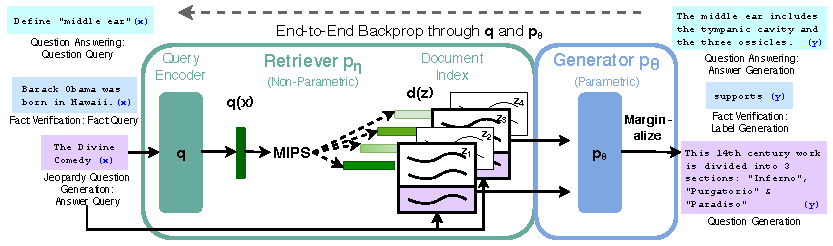
\includegraphics[width=\textwidth]{fig1_overview.pdf}
  \caption{Tổng quan về phương pháp của chúng tôi. Chúng tôi kết hợp một bộ
  truy xuất được huấn luyện trước (\emph{Bộ mã hoá truy vấn} + \emph{Chỉ mục
  tài liệu}) với một mô hình seq2seq được huấn luyện trước (\emph{Bộ sinh}) và
  tinh chỉnh đầu-cuối (end-to-end). Với truy vấn $x$, chúng tôi sử dụng Tìm
  kiếm Tích vô hướng Cực đại (Maximum Inner Product Search -- MIPS) để tìm
  top-K tài liệu $z_i$. Để đưa ra dự đoán cuối cùng $y$, chúng tôi xem $z$ như
  một biến ẩn và lấy biên (marginalize) trên các dự đoán seq2seq ứng với các
  tài liệu khác nhau.}
  \label{fig:overview}
\end{figure}

nhưng mới chỉ khám phá bài toán hỏi đáp trích xuất miền mở. Ở đây, chúng tôi
đưa bộ nhớ lai tham số và phi tham số vào ``con ngựa thồ của NLP'', tức là các
mô hình chuỗi-sang-chuỗi (sequence-to-sequence, seq2seq).

Chúng tôi trang bị cho các mô hình sinh có bộ nhớ tham số đã được huấn luyện
trước một bộ nhớ phi tham số thông qua một phương pháp tinh chỉnh đa dụng mà
chúng tôi gọi là sinh văn bản tăng cường truy xuất (RAG). Chúng tôi xây dựng
các mô hình RAG trong đó bộ nhớ tham số là một transformer seq2seq được huấn
luyện trước, và bộ nhớ phi tham số là một chỉ mục vectơ dày đặc của Wikipedia,
được truy cập bằng một bộ truy xuất nơ-ron được huấn luyện trước. Chúng tôi kết
hợp các thành phần này trong một mô hình xác suất được huấn luyện đầu-cuối
(Hình~\ref{fig:overview}). Bộ truy xuất (Dense Passage Retriever~\cite{b26},
từ đây gọi là DPR) cung cấp các tài liệu ẩn được điều kiện hoá theo đầu vào, và
mô hình seq2seq (BART~\cite{b32}) sau đó điều kiện hoá trên các tài liệu ẩn này
cùng với đầu vào để sinh ra đầu ra. Chúng tôi lấy biên các tài liệu ẩn bằng một
phép xấp xỉ top-K, hoặc theo từng đầu ra (giả định rằng cùng một tài liệu chịu
trách nhiệm cho tất cả các token) hoặc theo từng token (trong đó các tài liệu
khác nhau chịu trách nhiệm cho các token khác nhau). Giống như T5~\cite{b51}
hoặc BART, RAG có thể được tinh chỉnh trên bất kỳ tác vụ seq2seq nào, trong đó
cả bộ sinh và bộ truy xuất đều được học đồng thời.

Đã có nhiều công trình trước đây đề xuất các kiến trúc để làm giàu hệ thống
bằng bộ nhớ phi tham số, được huấn luyện từ đầu cho các tác vụ cụ thể, ví dụ
như mạng bộ nhớ (memory networks)~\cite{b64,b55}, mạng tăng cường ngăn xếp
(stack-augmented networks)~\cite{b25} và tầng bộ nhớ (memory
layers)~\cite{b30}. Ngược lại, chúng tôi khám phá một bối cảnh trong đó cả hai
thành phần bộ nhớ tham số và phi tham số đều được huấn luyện trước và được nạp
sẵn tri thức phong phú. Điều quan trọng là, nhờ sử dụng các cơ chế truy cập đã
được huấn luyện trước, khả năng truy cập tri thức đã có sẵn mà không cần huấn
luyện thêm.

Các kết quả của chúng tôi làm nổi bật lợi ích của việc kết hợp bộ nhớ tham số
và phi tham số với quá trình sinh cho các \emph{tác vụ đòi hỏi nhiều tri thức}
(knowledge-intensive tasks) --- những tác vụ mà con người khó có thể được kỳ
vọng thực hiện một cách hợp lý nếu không được tiếp cận một nguồn tri thức bên
ngoài. Các mô hình RAG của chúng tôi đạt kết quả tiên tiến nhất trên Natural
Questions mở~\cite{b29}, WebQuestions~\cite{b3} và CuratedTrec~\cite{b2}, và
vượt trội rõ rệt so với các phương pháp gần đây sử dụng các mục tiêu huấn luyện
trước chuyên biệt trên TriviaQA~\cite{b24}. Mặc dù đây là các tác vụ trích
xuất, chúng tôi nhận thấy rằng việc sinh không ràng buộc vượt trội các phương
pháp trích xuất trước đây. Đối với sinh văn bản đòi hỏi nhiều tri thức, chúng
tôi thử nghiệm với MS-MARCO~\cite{b1} và sinh câu hỏi Jeopardy, và nhận thấy
rằng các mô hình của chúng tôi sinh ra các câu trả lời đúng sự thật hơn, cụ thể
hơn và đa dạng hơn so với mô hình cơ sở BART. Đối với kiểm chứng sự thật
FEVER~\cite{b56}, chúng tôi đạt kết quả chỉ kém 4.3\% so với các mô hình
pipeline tiên tiến nhất vốn sử dụng giám sát truy xuất mạnh. Cuối cùng, chúng
tôi chứng minh rằng bộ nhớ phi tham số có thể được thay thế để cập nhật tri
thức của mô hình khi thế giới thay đổi.\footnote{Mã nguồn để chạy các thí
nghiệm với RAG đã được công bố mã nguồn mở như một phần của thư viện
HuggingFace Transformers~\cite{b66} và có thể tìm thấy tại
\url{https://github.com/huggingface/transformers/blob/master/examples/rag/}.
Bản demo tương tác của các mô hình RAG có thể được tìm thấy tại
\url{https://huggingface.co/rag/}}

% =====================================================================
\section{Phương pháp}
% =====================================================================
Chúng tôi khám phá các mô hình RAG, sử dụng chuỗi đầu vào $x$ để truy xuất các
tài liệu văn bản $z$ và dùng chúng làm ngữ cảnh bổ sung khi sinh chuỗi đích
$y$. Như thể hiện trong Hình~\ref{fig:overview}, các mô hình của chúng tôi tận
dụng hai thành phần: (i) một bộ truy xuất $p_\eta(z|x)$ với các tham số $\eta$,
trả về các phân phối (được cắt ngắn top-K) trên các đoạn văn bản khi cho một
truy vấn $x$, và (ii) một bộ sinh $p_\theta(y_i|x,z,y_{1:i-1})$ được tham số
hoá bởi $\theta$, sinh ra token hiện tại dựa trên ngữ cảnh gồm $i-1$ token
trước đó $y_{1:i-1}$, đầu vào gốc $x$ và một đoạn văn được truy xuất $z$.

Để huấn luyện bộ truy xuất và bộ sinh theo kiểu đầu-cuối, chúng tôi xem tài
liệu được truy xuất như một biến ẩn. Chúng tôi đề xuất hai mô hình lấy biên
trên các tài liệu ẩn theo những cách khác nhau để tạo ra một phân phối trên văn
bản được sinh. Trong cách tiếp cận thứ nhất, \emph{RAG-Sequence}, mô hình sử
dụng cùng một tài liệu để dự đoán mỗi token đích. Cách tiếp cận thứ hai,
\emph{RAG-Token}, có thể dự đoán mỗi token đích dựa trên một tài liệu khác
nhau. Trong phần tiếp theo, chúng tôi giới thiệu chính thức cả hai mô hình, sau
đó mô tả các thành phần $p_\eta$ và $p_\theta$, cũng như quy trình huấn luyện
và giải mã.

\subsection{Các mô hình}

\paragraph{Mô hình RAG-Sequence}
Mô hình RAG-Sequence sử dụng cùng một tài liệu được truy xuất để sinh toàn bộ
chuỗi. Về mặt kỹ thuật, nó xem tài liệu được truy xuất như một biến ẩn duy
nhất, được lấy biên để thu được xác suất seq2seq $p(y|x)$ thông qua một phép
xấp xỉ top-K. Cụ thể, top K tài liệu được truy xuất bằng bộ truy xuất, và bộ
sinh tính xác suất của chuỗi đầu ra cho mỗi tài liệu; sau đó các xác suất này
được lấy biên,
\[
  p_{\text{RAG-Sequence}}(y|x) \;\approx\; \sum_{z\in\topk} p_\eta(z|x)\,
  p_\theta(y|x,z) \;=\; \sum_{z\in\topk} p_\eta(z|x) \prod_{i}^{N}
  p_\theta(y_i|x,z,y_{1:i-1})
\]

\paragraph{Mô hình RAG-Token}
Trong mô hình RAG-Token, chúng ta có thể rút ra một tài liệu ẩn khác nhau cho
mỗi token đích và lấy biên tương ứng. Điều này cho phép bộ sinh chọn nội dung
từ nhiều tài liệu khi tạo ra câu trả lời. Cụ thể, top K tài liệu được truy xuất
bằng bộ truy xuất, sau đó bộ sinh tạo ra một phân phối cho token đầu ra tiếp
theo ứng với mỗi tài liệu, trước khi lấy biên, rồi lặp lại quá trình với token
đầu ra kế tiếp. Một cách hình thức, chúng tôi định nghĩa:
\[
  p_{\text{RAG-Token}}(y|x) \;\approx\; \prod_{i}^{N} \sum_{z\in\topk}
  p_\eta(z|x)\, p_\theta(y_i|x,z,y_{1:i-1})
\]

Cuối cùng, chúng tôi lưu ý rằng RAG có thể được dùng cho các tác vụ phân loại
chuỗi bằng cách xem lớp đích như một chuỗi đích có độ dài bằng một; khi đó
RAG-Sequence và RAG-Token là tương đương.

\subsection{Bộ truy xuất: DPR}

Thành phần truy xuất $p_\eta(z|x)$ dựa trên DPR~\cite{b26}. DPR tuân theo kiến
trúc bộ mã hoá kép (bi-encoder):
\[
  p_\eta(z|x) \propto \exp\!\left(\mathbf{d}(z)^{\top}\mathbf{q}(x)\right)
  \qquad
  \mathbf{d}(z) = \text{BERT}_d(z),\;\; \mathbf{q}(x) = \text{BERT}_q(x)
\]
trong đó $\mathbf{d}(z)$ là biểu diễn dày đặc của một tài liệu do bộ mã hoá tài
liệu BERT\textsubscript{BASE}~\cite{b8} tạo ra, và $\mathbf{q}(x)$ là biểu diễn
truy vấn do một bộ mã hoá truy vấn, cũng dựa trên BERT\textsubscript{BASE}, tạo
ra. Việc tính $\text{top-}k(p_\eta(\cdot|x))$, danh sách $k$ tài liệu $z$ có
xác suất tiên nghiệm $p_\eta(z|x)$ cao nhất, là một bài toán Tìm kiếm Tích vô
hướng Cực đại (MIPS), có thể được giải xấp xỉ trong thời gian dưới tuyến
tính~\cite{b23}. Chúng tôi sử dụng một bi-encoder đã được huấn luyện trước từ
DPR để khởi tạo bộ truy xuất và xây dựng chỉ mục tài liệu. Bộ truy xuất này đã
được huấn luyện để truy xuất các tài liệu chứa câu trả lời cho các câu hỏi của
TriviaQA~\cite{b24} và Natural Questions~\cite{b29}. Chúng tôi gọi chỉ mục tài
liệu là \emph{bộ nhớ phi tham số}.

\subsection{Bộ sinh: BART}

Thành phần sinh $p_\theta(y_i|x,z,y_{1:i-1})$ có thể được mô hình hoá bằng bất
kỳ kiến trúc mã hoá--giải mã (encoder-decoder) nào. Chúng tôi sử dụng
BART-large~\cite{b32}, một transformer seq2seq~\cite{b58} được huấn luyện trước
với 400 triệu tham số. Để kết hợp đầu vào $x$ với nội dung được truy xuất $z$
khi sinh bằng BART, chúng tôi chỉ đơn giản nối (concatenate) chúng lại với
nhau. BART được huấn luyện trước bằng một mục tiêu khử nhiễu (denoising) với
nhiều hàm gây nhiễu khác nhau. Nó đã đạt kết quả tiên tiến nhất trên nhiều tác
vụ sinh đa dạng và vượt trội các mô hình T5 có kích thước tương
đương~\cite{b32}. Từ đây, chúng tôi gọi các tham số $\theta$ của bộ sinh BART
là \emph{bộ nhớ tham số}.

\subsection{Huấn luyện}

Chúng tôi huấn luyện đồng thời các thành phần truy xuất và sinh mà không có bất
kỳ giám sát trực tiếp nào về việc tài liệu nào nên được truy xuất. Cho một tập
dữ liệu huấn luyện tinh chỉnh gồm các cặp đầu vào/đầu ra $(x_j, y_j)$, chúng
tôi cực tiểu hoá log-hợp lý biên âm (negative marginal log-likelihood) của mỗi
đích, $\sum_j -\log p(y_j|x_j)$, bằng phương pháp hạ gradient ngẫu nhiên với
Adam~\cite{b28}. Việc cập nhật bộ mã hoá tài liệu $\text{BERT}_d$ trong quá
trình huấn luyện rất tốn kém vì nó đòi hỏi chỉ mục tài liệu phải được cập nhật
định kỳ, như REALM đã làm trong giai đoạn huấn luyện trước~\cite{b20}. Chúng
tôi nhận thấy bước này không cần thiết để đạt hiệu năng cao, và giữ cố định bộ
mã hoá tài liệu (cùng chỉ mục), chỉ tinh chỉnh bộ mã hoá truy vấn
$\text{BERT}_q$ và bộ sinh BART.

\subsection{Giải mã}

Tại thời điểm kiểm thử, RAG-Sequence và RAG-Token đòi hỏi những cách khác nhau
để xấp xỉ $\operatorname*{arg\,max}_y p(y|x)$.

\paragraph{RAG-Token}
Mô hình RAG-Token có thể được xem như một bộ sinh seq2seq tự hồi quy
(autoregressive) tiêu chuẩn với xác suất chuyển tiếp:
\[
  p'_\theta(y_i|x,y_{1:i-1}) = \sum_{z\in\topk} p_\eta(z_i|x)\,
  p_\theta(y_i|x,z_i,y_{1:i-1})
\]
Để giải mã, chúng ta có thể đưa $p'_\theta(y_i|x,y_{1:i-1})$ vào một bộ giải
mã tìm kiếm chùm (beam search) tiêu chuẩn.

\paragraph{RAG-Sequence}
Với RAG-Sequence, hàm hợp lý $p(y|x)$ không tách được thành hợp lý theo từng
token thông thường, do đó ta không thể giải nó bằng một lần tìm kiếm chùm duy
nhất. Thay vào đó, chúng tôi chạy tìm kiếm chùm cho mỗi tài liệu $z$, chấm điểm
mỗi giả thuyết bằng $p_\theta(y_i|x,z,y_{1:i-1})$. Điều này tạo ra một tập giả
thuyết $Y$, trong đó một số giả thuyết có thể không xuất hiện trong chùm của
tất cả các tài liệu. Để ước lượng xác suất của một giả thuyết $y$, chúng tôi
chạy thêm một lượt truyền xuôi (forward pass) cho mỗi tài liệu $z$ mà $y$ không
xuất hiện trong chùm, nhân xác suất của bộ sinh với $p_\eta(z|x)$, rồi cộng các
xác suất qua các chùm để có xác suất biên. Chúng tôi gọi quy trình giải mã này
là ``Giải mã Kỹ lưỡng'' (Thorough Decoding). Với các chuỗi đầu ra dài hơn,
$|Y|$ có thể trở nên lớn, đòi hỏi nhiều lượt truyền xuôi. Để giải mã hiệu quả
hơn, chúng tôi có thể thực hiện thêm một phép xấp xỉ rằng
$p_\theta(y|x,z_i)\approx 0$ khi $y$ không được sinh ra trong quá trình tìm
kiếm chùm từ $x, z_i$. Điều này giúp tránh phải chạy thêm các lượt truyền xuôi
sau khi tập ứng viên $Y$ đã được sinh ra. Chúng tôi gọi quy trình giải mã này
là ``Giải mã Nhanh'' (Fast Decoding).

% =====================================================================
\section{Thí nghiệm}
% =====================================================================
Chúng tôi thử nghiệm RAG trên nhiều tác vụ đòi hỏi nhiều tri thức. Trong tất cả
các thí nghiệm, chúng tôi sử dụng một bản kết xuất (dump) Wikipedia duy nhất
làm nguồn tri thức phi tham số. Theo Lee và cộng sự~\cite{b31} và Karpukhin và
cộng sự~\cite{b26}, chúng tôi sử dụng bản kết xuất tháng 12 năm 2018. Mỗi bài
viết Wikipedia được chia thành các đoạn 100 từ không chồng lấn, tạo thành tổng
cộng 21 triệu tài liệu. Chúng tôi sử dụng bộ mã hoá tài liệu để tính vectơ
nhúng (embedding) cho mỗi tài liệu, và xây dựng một chỉ mục MIPS duy nhất bằng
FAISS~\cite{b23} với phép xấp xỉ Hierarchical Navigable Small World để truy
xuất nhanh~\cite{b37}. Trong quá trình huấn luyện, chúng tôi truy xuất top $k$
tài liệu cho mỗi truy vấn. Chúng tôi xét $k\in\{5,10\}$ khi huấn luyện và chọn
$k$ cho thời điểm kiểm thử dựa trên dữ liệu phát triển (dev). Tiếp theo, chúng
tôi trình bày chi tiết thí nghiệm cho từng tác vụ.

\subsection{Hỏi đáp miền mở}

Hỏi đáp (QA) miền mở là một ứng dụng thực tế quan trọng và là môi trường thử
nghiệm phổ biến cho các tác vụ đòi hỏi nhiều tri thức~\cite{b20}. Chúng tôi xem
câu hỏi và câu trả lời như các cặp văn bản đầu vào--đầu ra $(x,y)$ và huấn
luyện RAG bằng cách trực tiếp cực tiểu hoá log-hợp lý âm của câu trả lời. Chúng
tôi so sánh RAG với mô hình QA trích xuất phổ biến~\cite{b5,b7,b31,b26}, trong
đó câu trả lời là các đoạn (span) được trích ra từ tài liệu được truy xuất,
chủ yếu dựa vào tri thức phi tham số. Chúng tôi cũng so sánh với các phương
pháp ``QA sách đóng'' (Closed-Book QA)~\cite{b52}, vốn giống RAG ở chỗ sinh câu
trả lời, nhưng không khai thác truy xuất mà hoàn toàn dựa vào tri thức tham số.
Chúng tôi xét bốn tập dữ liệu QA miền mở phổ biến: Natural Questions
(NQ)~\cite{b29}, TriviaQA (TQA)~\cite{b24}, WebQuestions (WQ)~\cite{b3} và
CuratedTrec (CT)~\cite{b2}. Vì CT và WQ có kích thước nhỏ, chúng tôi làm theo
DPR~\cite{b26} bằng cách khởi tạo các mô hình CT và WQ từ mô hình RAG đã huấn
luyện trên NQ. Chúng tôi sử dụng cùng cách chia train/dev/test như các công
trình trước~\cite{b31,b26} và báo cáo điểm Khớp Chính xác (Exact Match -- EM).
Với TQA, để so sánh với T5~\cite{b52}, chúng tôi cũng đánh giá trên tập kiểm
thử TQA Wiki.

\subsection{Hỏi đáp trừu tượng}

Các mô hình RAG có thể vượt ra ngoài QA trích xuất đơn giản và trả lời câu hỏi
bằng văn bản sinh tự do, mang tính trừu tượng (abstractive). Để kiểm tra khả
năng sinh ngôn ngữ tự nhiên (NLG) của RAG trong bối cảnh đòi hỏi nhiều tri
thức, chúng tôi sử dụng tác vụ MSMARCO NLG v2.1~\cite{b43}. Tác vụ này bao gồm
các câu hỏi, mười đoạn văn chuẩn (gold) được truy xuất từ một công cụ tìm kiếm
cho mỗi câu hỏi, và một câu trả lời dạng câu hoàn chỉnh được chú thích từ các
đoạn văn được truy xuất. Chúng tôi không sử dụng các đoạn văn được cung cấp,
chỉ sử dụng câu hỏi và câu trả lời, để xem MSMARCO như một tác vụ QA trừu tượng
miền mở. MSMARCO có một số câu hỏi không thể trả lời sao cho khớp với câu trả
lời tham chiếu nếu không có quyền truy cập vào các đoạn văn chuẩn, chẳng hạn như
``What is the weather in Volcano, CA?'' (``Thời tiết ở Volcano, CA thế
nào?''), vì vậy hiệu năng sẽ thấp hơn khi không sử dụng các đoạn văn chuẩn.
Chúng tôi cũng lưu ý rằng một số câu hỏi MSMARCO không thể trả lời chỉ bằng
Wikipedia. Khi đó, RAG có thể dựa vào tri thức tham số để sinh ra những câu trả
lời hợp lý.

\subsection{Sinh câu hỏi Jeopardy}

Để đánh giá khả năng sinh của RAG trong bối cảnh không phải QA, chúng tôi
nghiên cứu bài toán sinh câu hỏi miền mở. Thay vì sử dụng câu hỏi từ các tác vụ
QA miền mở tiêu chuẩn, vốn thường gồm những câu hỏi ngắn và đơn giản, chúng tôi
đề xuất tác vụ khó hơn là sinh câu hỏi Jeopardy. Jeopardy là một định dạng khác
thường, trong đó người chơi phải cố gắng đoán một thực thể từ một sự kiện
(fact) về thực thể đó. Ví dụ, ``The World Cup'' là câu trả lời cho câu hỏi
``In 1986 Mexico scored as the first country to host this international sports
competition twice.'' (``Năm 1986, Mexico ghi dấu là quốc gia đầu tiên hai lần
đăng cai giải đấu thể thao quốc tế này.''). Vì các câu hỏi Jeopardy là những
phát biểu chính xác, mang tính sự thật, việc sinh câu hỏi Jeopardy khi được
điều kiện hoá trên thực thể trả lời của chúng tạo thành một tác vụ sinh đòi hỏi
nhiều tri thức đầy thách thức.

Chúng tôi sử dụng cách chia dữ liệu từ SearchQA~\cite{b10}, với 100 nghìn mẫu
huấn luyện, 14 nghìn mẫu phát triển và 27 nghìn mẫu kiểm thử. Vì đây là một tác
vụ mới, chúng tôi huấn luyện một mô hình BART để so sánh. Theo~\cite{b67},
chúng tôi đánh giá bằng thước đo Q-BLEU-1 được tinh chỉnh trên
SQuAD~\cite{b42}. Q-BLEU là một biến thể của BLEU với trọng số cao hơn cho việc
khớp các thực thể, và có tương quan với đánh giá của con người cao hơn so với
các thước đo tiêu chuẩn đối với bài toán sinh câu hỏi. Chúng tôi cũng thực hiện
hai đánh giá của con người, một để đánh giá tính xác thực của văn bản sinh, và
một cho tính cụ thể. Chúng tôi định nghĩa \emph{tính xác thực} (factuality) là
việc một phát biểu có thể được chứng thực bởi các nguồn bên ngoài đáng tin cậy
hay không, và \emph{tính cụ thể} (specificity) là mức độ phụ thuộc lẫn nhau cao
giữa đầu vào và đầu ra~\cite{b33}. Chúng tôi tuân theo thực hành tốt nhất và sử
dụng đánh giá so sánh theo cặp~\cite{b34}. Người đánh giá được cho xem một câu
trả lời và hai câu hỏi được sinh ra, một từ BART và một từ RAG. Sau đó họ được
yêu cầu chọn một trong bốn lựa chọn --- câu hỏi A tốt hơn, câu hỏi B tốt hơn,
cả hai đều tốt, hoặc không câu nào tốt.

\subsection{Kiểm chứng sự thật}

FEVER~\cite{b56} yêu cầu phân loại xem một khẳng định (claim) bằng ngôn ngữ tự
nhiên được Wikipedia ủng hộ hay bác bỏ, hoặc liệu có không đủ thông tin để
quyết định. Tác vụ này đòi hỏi truy xuất bằng chứng từ Wikipedia liên quan đến
khẳng định, sau đó suy luận trên bằng chứng này để phân loại khẳng định là
đúng, sai, hay không thể kiểm chứng chỉ từ Wikipedia. FEVER là một bài toán
truy xuất gắn liền với một tác vụ suy luận kéo theo (entailment) đầy thách
thức. Nó cũng là một môi trường thử nghiệm phù hợp để khám phá khả năng của các
mô hình RAG trong việc xử lý bài toán phân loại thay vì sinh. Chúng tôi ánh xạ
các nhãn lớp của FEVER (ủng hộ, bác bỏ, hoặc không đủ thông tin) thành các
token đầu ra đơn lẻ và huấn luyện trực tiếp với các cặp khẳng định--lớp. Điều
quan trọng là, không giống hầu hết các phương pháp khác cho FEVER, chúng tôi
không sử dụng giám sát trên bằng chứng được truy xuất. Trong nhiều ứng dụng
thực tế, tín hiệu giám sát truy xuất không có sẵn, và các mô hình không đòi hỏi
sự giám sát như vậy sẽ áp dụng được cho phạm vi tác vụ rộng hơn. Chúng tôi khám
phá hai biến thể: tác vụ phân loại 3 lớp tiêu chuẩn (ủng hộ/bác bỏ/không đủ
thông tin) và tác vụ 2 lớp (ủng hộ/bác bỏ) được nghiên cứu trong Thorne và
Vlachos~\cite{b57}. Trong cả hai trường hợp, chúng tôi báo cáo độ chính xác
nhãn.

% =====================================================================
\section{Kết quả}
% =====================================================================
\subsection{Hỏi đáp miền mở}

\begin{table}[t]
\centering
\begin{minipage}[t]{0.485\textwidth}
  \captionof{table}{Điểm kiểm thử QA miền mở. Với TQA, cột bên trái sử dụng tập
  kiểm thử tiêu chuẩn cho QA miền mở, cột bên phải sử dụng tập kiểm thử
  TQA-Wiki. Xem Phụ lục~\ref{app:odqa} để biết thêm chi tiết.}
  \label{tab:odqa}
  \vspace{2pt}
  \centering\small
  \setlength{\tabcolsep}{2.6pt}
  \begin{tabular}{@{}llcccc@{}}
    \toprule
     & Mô hình & NQ & TQA & WQ & CT\\
    \midrule
    \multirow{2}{*}{\makecell[l]{Sách\\đóng}}
     & T5-11B~\cite{b52} & 34.5 & -\,/50.1 & 37.4 & -\\
     & {\scriptsize T5-11B+SSM\cite{b52}} & 36.6 & -\,/60.5 & 44.7 & -\\
    \midrule
    \multirow{2}{*}{\makecell[l]{Sách\\mở}}
     & REALM~\cite{b20} & 40.4 & -\,/\,- & 40.7 & 46.8\\
     & DPR~\cite{b26} & 41.5 & \textbf{57.9}/\,- & 41.1 & 50.6\\
    \midrule
     & RAG-Token & 44.1 & 55.2/66.1 & \textbf{45.5} & 50.0\\
     & RAG-Seq. & \textbf{44.5} & 56.8/\textbf{68.0} & 45.2 & \textbf{52.2}\\
    \bottomrule
  \end{tabular}
\end{minipage}\hfill
\begin{minipage}[t]{0.485\textwidth}
  \captionof{table}{Điểm kiểm thử cho các tác vụ sinh và phân loại. SotA của
  MS-MARCO là~\cite{b4}, FEVER-3 là~\cite{b68} và FEVER-2 là~\cite{b57}.
  *Sử dụng ngữ cảnh/bằng chứng chuẩn (gold). Mô hình tốt nhất không truy cập
  dữ liệu chuẩn được gạch chân.}
  \label{tab:gen}
  \vspace{2pt}
  \centering\small
  \setlength{\tabcolsep}{2.4pt}
  \begin{tabular}{@{}lcccccc@{}}
    \toprule
    \multirow{2}{*}{Mô hình} & \multicolumn{2}{c}{Jeopardy} &
      \multicolumn{2}{c}{MSMARCO} & FVR3 & FVR2\\
     & B-1 & QB-1 & R-L & B-1 & \multicolumn{2}{c}{\makecell{Đ.c.x. nhãn}}\\
    \midrule
    SotA & - & - & \textbf{49.8}* & \textbf{49.9}* & \textbf{76.8} &
      \textbf{92.2}*\\
    \midrule
    BART & 15.1 & 19.7 & 38.2 & 41.6 & 64.0 & 81.1\\
    \midrule
    RAG-Tok. & \textbf{17.3} & \textbf{22.2} & 40.1 & 41.5 &
      \multirow{2}{*}{72.5} & \multirow{2}{*}{\underline{89.5}}\\
    RAG-Seq. & 14.7 & 21.4 & \underline{40.8} & \underline{44.2} & & \\
    \bottomrule
  \end{tabular}\\[2pt]
  {\footnotesize (Đ.c.x. nhãn = độ chính xác nhãn)}
\end{minipage}
\end{table}

Bảng~\ref{tab:odqa} trình bày kết quả của RAG cùng với các mô hình tiên tiến
nhất. Trên cả bốn tác vụ QA miền mở, RAG thiết lập một kết quả tiên tiến nhất
mới (với TQA thì chỉ trên tập chia có thể so sánh với T5). RAG kết hợp sự linh
hoạt trong việc sinh của các phương pháp ``sách đóng'' (chỉ tham số) với hiệu
năng của các phương pháp ``sách mở'' dựa trên truy xuất. Không giống REALM và
T5+SSM, RAG đạt kết quả mạnh mà không cần giai đoạn huấn luyện trước ``che mặt
nạ các đoạn nổi bật'' (salient span masking) tốn kém và chuyên
biệt~\cite{b20}. Đáng chú ý là bộ truy xuất của RAG được khởi tạo từ bộ truy
xuất của DPR, vốn sử dụng giám sát truy xuất trên Natural Questions và
TriviaQA. RAG cho kết quả tốt hơn so với hệ thống QA của DPR, vốn sử dụng một
``bộ mã hoá chéo'' (cross-encoder) dựa trên BERT để xếp hạng lại tài liệu, cùng
với một bộ đọc trích xuất (extractive reader). RAG chứng minh rằng cả bộ xếp
hạng lại (re-ranker) lẫn bộ đọc trích xuất đều không cần thiết để đạt hiệu năng
tiên tiến nhất.

Có nhiều lợi thế khi sinh câu trả lời ngay cả khi có thể trích xuất chúng.
Những tài liệu chứa manh mối về câu trả lời nhưng không chứa nguyên văn câu trả
lời vẫn có thể góp phần vào việc sinh ra câu trả lời đúng, điều không thể thực
hiện được với các phương pháp trích xuất tiêu chuẩn, dẫn đến việc lấy biên trên
các tài liệu hiệu quả hơn. Hơn nữa, RAG có thể sinh ra câu trả lời đúng ngay cả
khi câu trả lời đúng không nằm trong bất kỳ tài liệu được truy xuất nào, đạt độ
chính xác 11.8\% trong những trường hợp như vậy đối với NQ, trong khi một mô
hình trích xuất sẽ đạt 0\%.

\subsection{Hỏi đáp trừu tượng}

Như thể hiện trong Bảng~\ref{tab:gen}, RAG-Sequence vượt trội BART trên Open
MS-MARCO NLG 2.6 điểm Bleu và 2.6 điểm Rouge-L. RAG tiệm cận hiệu năng của mô
hình tiên tiến nhất, điều này rất ấn tượng khi xét rằng (i) các mô hình đó truy
cập các đoạn văn chuẩn chứa thông tin cụ thể cần thiết để sinh câu trả lời tham
chiếu, (ii) nhiều câu hỏi không thể trả lời nếu không có các đoạn văn chuẩn, và
(iii) không phải câu hỏi nào cũng có thể trả lời chỉ từ Wikipedia.
Bảng~\ref{tab:examples} trình bày một số câu trả lời được sinh bởi các mô hình
của chúng tôi. Về mặt định tính, chúng tôi nhận thấy các mô hình RAG ít bị ảo
giác hơn và sinh văn bản đúng sự thật thường xuyên hơn BART. Ở phần sau, chúng
tôi cũng cho thấy văn bản do RAG sinh ra đa dạng hơn văn bản do BART sinh ra
(xem §\ref{sec:additional}).

\subsection{Sinh câu hỏi Jeopardy}
\label{sec:jeopardy}

Bảng~\ref{tab:gen} cho thấy RAG-Token hoạt động tốt hơn RAG-Sequence trong việc
sinh câu hỏi Jeopardy, và cả hai mô hình đều vượt trội BART trên Q-BLEU-1.
Bảng~\ref{tab:human} trình bày kết quả đánh giá của con người trên 452 cặp văn
bản sinh từ BART và RAG-Token. Người đánh giá cho biết BART đúng sự thật hơn
RAG chỉ trong 7.1\% trường hợp, trong khi RAG đúng sự thật hơn trong 42.7\%
trường hợp, và cả RAG lẫn BART đều đúng sự thật trong thêm 17\% trường hợp nữa,
chứng tỏ rõ ràng hiệu quả của RAG trên tác vụ này so với một mô hình sinh tiên
tiến nhất. Người đánh giá cũng nhận thấy văn bản do RAG sinh ra cụ thể hơn với
cách biệt lớn. Bảng~\ref{tab:examples} trình bày các văn bản sinh điển hình từ
mỗi mô hình.

Các câu hỏi Jeopardy thường chứa hai mẩu thông tin riêng biệt, và RAG-Token có
thể hoạt động tốt nhất vì nó có thể sinh ra câu trả lời kết hợp nội dung từ
nhiều tài liệu. Hình~\ref{fig:posterior} minh hoạ một ví dụ. Khi sinh ``Sun'',
phân phối hậu nghiệm (posterior) cao đối với tài liệu 2, tài liệu có đề cập đến
``The Sun Also Rises''. Tương tự, tài liệu 1 chiếm ưu thế trong phân phối hậu
nghiệm khi ``A Farewell to Arms'' được sinh ra. Điều thú vị là, sau khi token
đầu tiên của mỗi tên sách được sinh ra, phân phối hậu nghiệm trên các tài liệu
trở nên phẳng. Quan sát này gợi ý rằng bộ sinh có thể hoàn thành các tựa sách
mà không phụ thuộc vào các tài liệu cụ thể. Nói cách khác, tri thức tham số của
mô hình là đủ để hoàn thành các tựa sách. Chúng tôi tìm thấy bằng chứng cho giả
thuyết này bằng cách đưa cho mô hình cơ sở chỉ-BART phần giải mã dở dang
\gen{"The Sun}. BART hoàn thành việc sinh thành \gen{"The Sun Also Rises" is a
novel by this author of "The Sun Also Rises"}, cho thấy tựa sách ``The Sun Also
Rises'' được lưu trữ trong các tham số của BART. Tương tự, BART sẽ hoàn thành
phần giải mã dở dang \gen{"The Sun Also Rises" is a novel by this author of "A}
thành \gen{"The Sun Also Rises" is a novel by this author of "A Farewell to
Arms"}.\tnote{Các chuỗi đơn cách là đầu ra nguyên văn (tiếng Anh) của mô hình.
\gen{"The Sun Also Rises" is a novel by this author of "\ldots"} nghĩa là
``‘The Sun Also Rises’ (\emph{Mặt trời vẫn mọc}) là một tiểu thuyết của tác giả
của ‘\ldots’''; ``A Farewell to Arms'' là tiểu thuyết \emph{Giã từ vũ khí}.} Ví
dụ này cho thấy bộ nhớ tham số và phi tham số \emph{phối hợp với nhau} như thế
nào --- thành phần phi tham số giúp định hướng quá trình sinh, khơi gợi những
tri thức cụ thể được lưu trữ trong bộ nhớ tham số.

\subsection{Kiểm chứng sự thật}

Bảng~\ref{tab:gen} trình bày kết quả của chúng tôi trên FEVER. Với phân loại 3
lớp, điểm của RAG chỉ kém 4.3\% so với các mô hình tiên tiến nhất, vốn là những
hệ thống pipeline phức tạp với kiến trúc chuyên biệt cho miền và nhiều công sức
kỹ thuật, được huấn luyện với giám sát truy xuất trung gian mà RAG không cần
đến.

\begin{figure}[t]
  \centering
  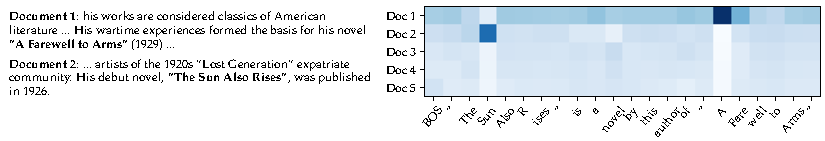
\includegraphics[width=\textwidth]{fig2_posterior.pdf}
  \caption{Phân phối hậu nghiệm trên tài liệu $p(z_i|x,y_i,y_{-i})$ của
  RAG-Token cho mỗi token được sinh, với đầu vào ``Hemingway'' cho tác vụ sinh
  Jeopardy với 5 tài liệu được truy xuất. Phân phối hậu nghiệm của tài liệu 1
  cao khi sinh ``A Farewell to Arms'' và của tài liệu 2 khi sinh ``The Sun Also
  Rises''.\\[3pt]
  {\small\textit{Ghi chú của người dịch --- nội dung hai tài liệu trong hình:}
  \textbf{Tài liệu 1}: các tác phẩm của ông được coi là kinh điển của văn học
  Mỹ \ldots\ Những trải nghiệm thời chiến của ông là cơ sở cho tiểu thuyết
  \textbf{``A Farewell to Arms''} (1929) \ldots\ \textbf{Tài liệu 2}: \ldots\
  các nghệ sĩ của cộng đồng kiều dân ``Thế hệ đã mất'' (Lost Generation) những
  năm 1920. Tiểu thuyết đầu tay của ông, \textbf{``The Sun Also Rises''}, được
  xuất bản năm 1926.}}
  \label{fig:posterior}
\end{figure}

\begin{table}[t]
\caption{Ví dụ từ các tác vụ sinh. Các mô hình RAG sinh ra câu trả lời cụ thể
hơn và chính xác hơn về mặt sự thật. `?' biểu thị câu trả lời sai sự thật, *
biểu thị câu trả lời đúng một phần. (Dòng in nghiêng màu xám là bản dịch tiếng
Việt của người dịch; văn bản gốc do mô hình sinh ra bằng tiếng Anh.)}
\label{tab:examples}
\centering\footnotesize
\setlength{\tabcolsep}{3pt}
\renewcommand{\arraystretch}{1.05}
\begin{tabularx}{\textwidth}{@{}>{\raggedright}p{1.25cm}>{\raggedright}p{1.75cm}l
    >{\raggedright\arraybackslash}X@{}}
  \toprule
  Tác vụ & Đầu vào & Mô hình & Văn bản được sinh\\
  \midrule
  \multirow{6}{=}{MS-MARCO}
  & \multirow{3}{=}{define middle ear\newline{\color{black!60}\itshape
      (định nghĩa tai giữa)}}
    & BART & $^?$The middle ear is the part of the ear between the middle ear
      and the nose.\vi{Tai giữa là phần của tai nằm giữa tai giữa và mũi.}\\
  & & RAG-T & The middle ear is the portion of the ear internal to the
      eardrum.\vi{Tai giữa là phần của tai nằm phía trong màng nhĩ.}\\
  & & RAG-S & The middle ear includes the tympanic cavity and the three
      ossicles.\vi{Tai giữa bao gồm hòm nhĩ và ba xương con.}\\
  \cmidrule(l){2-4}
  & \multirow{3}{=}{what currency needed in scotland\newline
      {\color{black!60}\itshape (ở Scotland cần dùng tiền tệ gì)}}
    & BART & The currency needed in Scotland is Pound sterling.\vi{Tiền tệ
      cần dùng ở Scotland là bảng Anh (Pound sterling).}\\
  & & RAG-T & Pound is the currency needed in Scotland.\vi{Bảng là tiền tệ
      cần dùng ở Scotland.}\\
  & & RAG-S & The currency needed in Scotland is the pound sterling.\vi{Tiền
      tệ cần dùng ở Scotland là đồng bảng Anh.}\\
  \midrule
  \multirow{6}{=}{Sinh câu hỏi Jeopardy}
  & \multirow{3}{=}{Washington}
    & BART & $^?$This state has the largest number of counties in the
      U.S.\vi{Bang này có số hạt nhiều nhất nước Mỹ.}\\
  & & RAG-T & It's the only U.S. state named for a U.S. president\vi{Đây là
      bang duy nhất của Mỹ được đặt theo tên một tổng thống Mỹ}\\
  & & RAG-S & It's the state where you'll find Mount Rainier National
      Park\vi{Đây là bang nơi bạn sẽ tìm thấy Vườn quốc gia Núi Rainier}\\
  \cmidrule(l){2-4}
  & \multirow{3}{=}{The Divine Comedy\newline{\color{black!60}\itshape
      (Thần khúc)}}
    & BART & $^*$This epic poem by Dante is divided into 3 parts: the Inferno,
      the Purgatorio \& the Purgatorio\vi{Bản sử thi này của Dante được chia
      thành 3 phần: Inferno, Purgatorio \& Purgatorio}\\
  & & RAG-T & Dante's ``Inferno'' is the first part of this epic poem\vi{“Inferno”
      (Địa ngục) của Dante là phần đầu tiên của bản sử thi này}\\
  & & RAG-S & This 14th century work is divided into 3 sections: ``Inferno'',
      ``Purgatorio'' \& ``Paradiso''\vi{Tác phẩm thế kỷ 14 này được chia thành 3
      phần: “Inferno”, “Purgatorio” \& “Paradiso”}\\
  \bottomrule
\end{tabularx}
\end{table}

Với phân loại 2 lớp, chúng tôi so sánh với Thorne và Vlachos~\cite{b57}, những
người huấn luyện RoBERTa~\cite{b35} để phân loại khẳng định là đúng hay sai khi
được cho câu bằng chứng chuẩn. RAG đạt độ chính xác chỉ kém 2.7\% so với mô
hình này, mặc dù chỉ được cung cấp khẳng định và tự truy xuất bằng chứng của
riêng mình. Chúng tôi cũng phân tích xem các tài liệu được RAG truy xuất có
tương ứng với các tài liệu được chú thích là bằng chứng chuẩn trong FEVER hay
không. Chúng tôi tính mức độ trùng lặp về tiêu đề bài viết giữa top $k$ tài
liệu được RAG truy xuất và các chú thích bằng chứng chuẩn. Chúng tôi nhận thấy
tài liệu được truy xuất đứng đầu thuộc về một bài viết chuẩn trong 71\% trường
hợp, và một bài viết chuẩn có mặt trong top 10 bài viết được truy xuất trong
90\% trường hợp.

\subsection{Kết quả bổ sung}
\label{sec:additional}

\paragraph{Tính đa dạng của văn bản sinh}
Mục~\ref{sec:jeopardy} cho thấy các mô hình RAG đúng sự thật hơn và cụ thể hơn
BART trong việc sinh câu hỏi Jeopardy. Theo các công trình gần đây về giải mã
thúc đẩy tính đa dạng~\cite{b33,b59,b39}, chúng tôi cũng khảo sát tính đa dạng
của văn bản sinh bằng cách tính tỷ lệ giữa số n-gram khác nhau và tổng số
n-gram được sinh bởi các mô hình khác nhau. Bảng~\ref{tab:diversity} cho thấy
văn bản sinh của RAG-Sequence đa dạng hơn của RAG-Token, và cả hai đều đa dạng
hơn đáng kể so với BART mà không cần bất kỳ phương pháp giải mã thúc đẩy đa
dạng nào.

\paragraph{Thí nghiệm cắt bỏ thành phần truy xuất (Retrieval Ablations)}
Một đặc điểm then chốt của RAG là học cách truy xuất thông tin liên quan cho
tác vụ. Để đánh giá hiệu quả của cơ chế truy xuất, chúng tôi chạy các thí
nghiệm cắt bỏ (ablation) trong đó bộ truy xuất bị đóng băng trong quá trình
huấn luyện. Như thể hiện trong Bảng~\ref{tab:ablation}, truy xuất được học giúp
cải thiện kết quả trên tất cả các tác vụ.

Chúng tôi so sánh bộ truy xuất dày đặc của RAG với bộ truy xuất
BM25~\cite{b53} dựa trên sự trùng lặp từ. Ở đây, chúng tôi thay thế bộ truy
xuất của RAG bằng một hệ thống BM25 cố định, và sử dụng điểm truy xuất BM25 làm
logit khi tính $p(z|x)$. Bảng~\ref{tab:ablation} trình bày kết quả. Với FEVER,
BM25 hoạt động tốt nhất, có lẽ vì các khẳng định trong FEVER tập trung nhiều
vào thực thể và do đó rất phù hợp với truy xuất dựa trên trùng lặp từ. Truy
xuất khả vi cải thiện kết quả trên tất cả các tác vụ khác, đặc biệt là với QA
miền mở, nơi nó đóng vai trò then chốt.

\paragraph{Hoán đổi nóng chỉ mục (Index hot-swapping)}
Một lợi thế của các mô hình có bộ nhớ phi tham số như RAG là tri thức có thể dễ
dàng được cập nhật tại thời điểm kiểm thử. Các mô hình chỉ có tham số như T5
hay BART cần được huấn luyện thêm để cập nhật hành vi khi thế giới thay đổi. Để
minh chứng, chúng tôi xây dựng một chỉ mục sử dụng bản kết xuất Wikipedia của
DrQA~\cite{b5} từ tháng 12 năm 2016 và so sánh đầu ra của RAG khi dùng chỉ mục
này với chỉ mục mới hơn trong các kết quả chính của chúng tôi (tháng 12 năm
2018). Chúng tôi chuẩn bị một danh sách 82 nhà lãnh đạo thế giới đã thay đổi

\begin{table}[t]
\centering
\begin{minipage}[t]{0.47\textwidth}
  \captionof{table}{Đánh giá của con người cho tác vụ sinh câu hỏi Jeopardy.}
  \label{tab:human}
  \vspace{2pt}
  \centering\small
  \begin{tabular}{@{}lcc@{}}
    \toprule
     & Tính xác thực & Tính cụ thể\\
    \midrule
    BART tốt hơn & 7.1\% & 16.8\%\\
    RAG tốt hơn & \textbf{42.7\%} & \textbf{37.4\%}\\
    Cả hai đều tốt & 11.7\% & 11.8\%\\
    Cả hai đều kém & 17.7\% & 6.9\%\\
    Không có đa số & 20.8\% & 20.1\%\\
    \bottomrule
  \end{tabular}
\end{minipage}\hfill
\begin{minipage}[t]{0.49\textwidth}
  \captionof{table}{Tỷ lệ giữa số tri-gram khác nhau và tổng số tri-gram cho
  các tác vụ sinh.}
  \label{tab:diversity}
  \vspace{2pt}
  \centering\small
  \begin{tabular}{@{}lcc@{}}
    \toprule
     & MSMARCO & Jeopardy QGen\\
    \midrule
    Chuẩn (Gold) & 89.6\% & 90.0\%\\
    BART & 70.7\% & 32.4\%\\
    RAG-Token & 77.8\% & 46.8\%\\
    RAG-Seq. & 83.5\% & 53.8\%\\
    \bottomrule
  \end{tabular}
\end{minipage}

\vspace{14pt}
\captionof{table}{Các thí nghiệm cắt bỏ trên tập phát triển (dev). Vì FEVER là
một tác vụ phân loại, hai mô hình RAG là tương đương.}
\label{tab:ablation}
\vspace{2pt}
\small
\setlength{\tabcolsep}{3.6pt}
\begin{tabular}{@{}lcccc@{\hspace{9pt}}cc@{\hspace{9pt}}cc@{\hspace{9pt}}cc@{}}
  \toprule
  \multirow{2}{*}{Mô hình} & NQ & TQA & WQ & CT &
    \multicolumn{2}{c}{Jeopardy-QGen} & \multicolumn{2}{c}{MSMarco} &
    FVR-3 & FVR-2\\
   & \multicolumn{4}{c}{Khớp chính xác} & B-1 & QB-1 & R-L & B-1 &
    \multicolumn{2}{c}{Độ chính xác nhãn}\\
  \midrule
  RAG-Token-BM25 & 29.7 & 41.5 & 32.1 & 33.1 & 17.5 & 22.3 & 55.5 & 48.4 &
    \multirow{2}{*}{\textbf{75.1}} & \multirow{2}{*}{\textbf{91.6}}\\
  RAG-Sequence-BM25 & 31.8 & 44.1 & 36.6 & 33.8 & 11.1 & 19.5 & 56.5 & 46.9
    & & \\
  \midrule
  RAG-Token-Frozen & 37.8 & 50.1 & 37.1 & 51.1 & 16.7 & 21.7 & 55.9 & 49.4 &
    \multirow{2}{*}{72.9} & \multirow{2}{*}{89.4}\\
  RAG-Sequence-Frozen & 41.2 & 52.1 & 41.8 & 52.6 & 11.8 & 19.6 & 56.7 & 47.3
    & & \\
  \midrule
  RAG-Token & 43.5 & 54.8 & \textbf{46.5} & 51.9 & \textbf{17.9} &
    \textbf{22.6} & 56.2 & \textbf{49.4} &
    \multirow{2}{*}{74.5} & \multirow{2}{*}{90.6}\\
  RAG-Sequence & \textbf{44.0} & \textbf{55.8} & 44.9 & \textbf{53.4} & 15.3 &
    21.5 & \textbf{57.2} & 47.5 & & \\
  \bottomrule
\end{tabular}
\end{table}

giữa hai thời điểm này và sử dụng mẫu câu ``Who is \{position\}?'' (``Ai là
\{chức vụ\}?'', ví dụ ``Who is the President of Peru?'' --- ``Ai là Tổng thống
Peru?'') để truy vấn mô hình RAG trên NQ của chúng tôi với mỗi chỉ mục. RAG trả
lời đúng 70\% khi dùng chỉ mục 2016 cho các nhà lãnh đạo thế giới năm 2016 và
68\% khi dùng chỉ mục 2018 cho các nhà lãnh đạo thế giới năm 2018. Độ chính xác
với các chỉ mục không khớp thì thấp (12\% với chỉ mục 2018 và các nhà lãnh đạo
2016, 4\% với chỉ mục 2016 và các nhà lãnh đạo 2018). Điều này cho thấy chúng
ta có thể cập nhật tri thức về thế giới của RAG chỉ bằng cách thay thế bộ nhớ
phi tham số của nó.

\paragraph{Ảnh hưởng của việc truy xuất nhiều tài liệu hơn}
Các mô hình được huấn luyện với 5 hoặc 10 tài liệu ẩn được truy xuất, và chúng
tôi không quan sát thấy khác biệt đáng kể về hiệu năng giữa hai thiết lập này.
Chúng tôi có thể linh hoạt điều chỉnh số lượng tài liệu được truy xuất tại thời
điểm kiểm thử, điều này có thể ảnh hưởng đến hiệu năng và thời gian chạy.
Hình~\ref{fig:kdocs} (trái) cho thấy việc truy xuất nhiều tài liệu hơn tại
thời điểm kiểm thử cải thiện đơn điệu kết quả QA miền mở của RAG-Sequence,
nhưng hiệu năng của RAG-Token đạt đỉnh ở 10 tài liệu được truy xuất.
Hình~\ref{fig:kdocs} (phải) cho thấy việc truy xuất nhiều tài liệu hơn dẫn đến
Rouge-L cao hơn cho RAG-Token nhưng phải đánh đổi bằng Bleu-1, trong khi ảnh
hưởng này ít rõ rệt hơn đối với RAG-Sequence.

\begin{figure}[t]
  \centering
  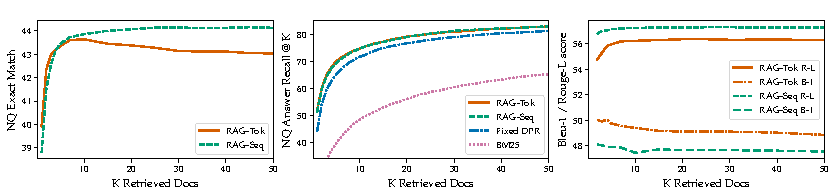
\includegraphics[width=\textwidth]{fig3_kdocs.pdf}
  \caption{Trái: Hiệu năng trên NQ khi truy xuất nhiều tài liệu hơn. Giữa: Độ
  phủ (recall) truy xuất trên NQ. Phải: Bleu-1 và Rouge-L trên MS-MARCO khi
  truy xuất nhiều tài liệu hơn.}
  \label{fig:kdocs}
\end{figure}

% =====================================================================
\section{Các công trình liên quan}
% =====================================================================
\paragraph{Truy xuất cho từng tác vụ đơn lẻ}
Các công trình trước đây đã chỉ ra rằng truy xuất cải thiện hiệu năng trên
nhiều tác vụ NLP khác nhau khi được xem xét riêng lẻ. Các tác vụ đó bao gồm hỏi
đáp miền mở~\cite{b5,b29}, kiểm tra sự thật~\cite{b56}, hoàn thiện sự kiện
(fact completion)~\cite{b48}, hỏi đáp dạng dài~\cite{b12}, sinh bài viết
Wikipedia~\cite{b36}, hội thoại~\cite{b41,b65,b9,b13}, dịch máy~\cite{b17}, và
mô hình hoá ngôn ngữ~\cite{b19,b27}. Công trình của chúng tôi hợp nhất những
thành công trước đây trong việc tích hợp truy xuất vào từng tác vụ riêng lẻ,
cho thấy rằng một kiến trúc duy nhất dựa trên truy xuất có khả năng đạt hiệu
năng mạnh trên nhiều tác vụ.

\paragraph{Kiến trúc đa dụng cho NLP}
Các công trình trước đây về kiến trúc đa dụng cho các tác vụ NLP đã đạt thành
công lớn mà không cần sử dụng truy xuất. Một mô hình ngôn ngữ duy nhất được
huấn luyện trước đã được chứng minh là đạt hiệu năng mạnh trên nhiều tác vụ
phân loại trong các bộ benchmark GLUE~\cite{b60,b61} sau khi tinh
chỉnh~\cite{b49,b8}. GPT-2~\cite{b50} sau đó cho thấy rằng một mô hình ngôn ngữ
duy nhất, từ trái sang phải, được huấn luyện trước có thể đạt hiệu năng mạnh
trên cả các tác vụ phân biệt (discriminative) lẫn tác vụ sinh (generative). Để
cải thiện hơn nữa, BART~\cite{b32} và T5~\cite{b51,b52} đề xuất một mô hình mã
hoá--giải mã duy nhất, được huấn luyện trước, tận dụng cơ chế chú ý hai chiều
để đạt hiệu năng mạnh hơn trên các tác vụ phân biệt và tác vụ sinh. Công trình
của chúng tôi nhằm mở rộng không gian các tác vụ khả thi với một kiến trúc
thống nhất duy nhất, bằng cách học một mô-đun truy xuất để tăng cường cho các
mô hình ngôn ngữ sinh đã được huấn luyện trước.

\paragraph{Truy xuất được học}
Có nhiều công trình đáng kể về việc học cách truy xuất tài liệu trong lĩnh vực
truy xuất thông tin, gần đây hơn là với các mô hình ngôn ngữ nơ-ron được huấn
luyện trước~\cite{b44,b26} tương tự như của chúng tôi. Một số công trình tối ưu
hoá mô-đun truy xuất để hỗ trợ một tác vụ hạ nguồn cụ thể như hỏi đáp, sử dụng
tìm kiếm~\cite{b46}, học tăng cường~\cite{b6,b63,b62}, hoặc một cách tiếp cận
biến ẩn~\cite{b31,b20} như trong công trình của chúng tôi. Những thành công này
tận dụng các kiến trúc dựa trên truy xuất và kỹ thuật tối ưu hoá khác nhau để
đạt hiệu năng mạnh trên một tác vụ duy nhất, trong khi chúng tôi cho thấy rằng
một kiến trúc duy nhất dựa trên truy xuất có thể được tinh chỉnh để đạt hiệu
năng mạnh trên nhiều tác vụ khác nhau.

\paragraph{Kiến trúc dựa trên bộ nhớ}
Chỉ mục tài liệu của chúng tôi có thể được xem như một bộ nhớ ngoài lớn để các
mạng nơ-ron chú ý (attend) tới, tương tự như mạng bộ nhớ~\cite{b64,b55}. Một
công trình đồng thời~\cite{b14} học cách truy xuất một vectơ nhúng đã huấn
luyện cho mỗi thực thể trong đầu vào, thay vì truy xuất văn bản thô như trong
công trình của chúng tôi. Các công trình khác cải thiện khả năng của mô hình
hội thoại trong việc sinh văn bản đúng sự thật bằng cách chú ý tới các vectơ
nhúng sự kiện~\cite{b15,b13}. Một đặc điểm then chốt của bộ nhớ của chúng tôi
là nó bao gồm văn bản thô thay vì các biểu diễn phân tán, điều này làm cho bộ
nhớ vừa (i) con người đọc được, mang lại một dạng khả năng diễn giải cho mô
hình, vừa (ii) con người viết được, cho phép chúng tôi cập nhật động bộ nhớ của
mô hình bằng cách chỉnh sửa chỉ mục tài liệu. Cách tiếp cận này cũng đã được sử
dụng trong hội thoại đòi hỏi nhiều tri thức, trong đó các bộ sinh được điều
kiện hoá trực tiếp trên văn bản được truy xuất, mặc dù văn bản này thu được
thông qua TF-IDF thay vì truy xuất được học đầu-cuối~\cite{b9}.

\paragraph{Các phương pháp Truy xuất-và-Chỉnh sửa (Retrieve-and-Edit)}
Phương pháp của chúng tôi có một số điểm tương đồng với các phương pháp kiểu
truy xuất-và-chỉnh sửa, trong đó một cặp đầu vào--đầu ra huấn luyện tương tự
được truy xuất cho một đầu vào cho trước, rồi được chỉnh sửa để tạo ra đầu ra
cuối cùng. Những phương pháp này đã chứng tỏ thành công trong nhiều lĩnh vực
bao gồm Dịch máy~\cite{b18,b22} và Phân tích ngữ nghĩa (Semantic
Parsing)~\cite{b21}. Cách tiếp cận của chúng tôi có một số khác biệt, bao gồm
việc ít chú trọng vào chỉnh sửa nhẹ một mục được truy xuất, mà chú trọng vào
việc tổng hợp nội dung từ nhiều mẩu nội dung được truy xuất, cũng như học truy
xuất ẩn, và truy xuất các tài liệu bằng chứng thay vì các cặp huấn luyện liên
quan. Dù vậy, các kỹ thuật RAG có thể hoạt động tốt trong những bối cảnh này và
có thể là một hướng nghiên cứu tương lai đầy hứa hẹn.

% =====================================================================
\section{Thảo luận}
% =====================================================================
Trong công trình này, chúng tôi đã trình bày các mô hình sinh lai có quyền truy
cập vào bộ nhớ tham số và phi tham số. Chúng tôi đã cho thấy các mô hình RAG
của mình đạt kết quả tiên tiến nhất trên QA miền mở. Chúng tôi nhận thấy mọi
người ưa thích văn bản do RAG sinh ra hơn so với BART thuần tham số, đánh giá
RAG là đúng sự thật hơn và cụ thể hơn. Chúng tôi đã tiến hành một khảo sát kỹ
lưỡng về thành phần truy xuất được học, xác nhận hiệu quả của nó, và minh hoạ
cách chỉ mục truy xuất có thể được hoán đổi nóng để cập nhật mô hình mà không
cần huấn luyện lại. Trong tương lai, có thể sẽ hữu ích nếu nghiên cứu liệu hai
thành phần có thể được huấn luyện trước đồng thời từ đầu hay không, với một mục
tiêu khử nhiễu tương tự BART hoặc một mục tiêu khác. Công trình của chúng tôi
mở ra những hướng nghiên cứu mới về cách bộ nhớ tham số và phi tham số tương
tác với nhau và cách kết hợp chúng hiệu quả nhất, cho thấy triển vọng được áp
dụng vào nhiều tác vụ NLP khác nhau.

% =====================================================================
\section*{Tác động rộng hơn}
% =====================================================================
Công trình này mang lại một số lợi ích tích cực cho xã hội so với các công
trình trước đây: việc nó được neo chặt hơn vào tri thức thực tế (trong trường
hợp này là Wikipedia) khiến nó ít ``ảo giác'' hơn, với văn bản sinh ra đúng sự
thật hơn, đồng thời mang lại khả năng kiểm soát và diễn giải tốt hơn. RAG có
thể được sử dụng trong nhiều kịch bản khác nhau mang lại lợi ích trực tiếp cho
xã hội, ví dụ bằng cách trang bị cho nó một chỉ mục y khoa và đặt các câu hỏi
miền mở về chủ đề đó, hoặc bằng cách giúp mọi người làm việc hiệu quả hơn.

Đi kèm với những lợi thế này cũng là những nhược điểm tiềm ẩn: Wikipedia, hay
bất kỳ nguồn tri thức bên ngoài tiềm năng nào, có lẽ sẽ không bao giờ hoàn toàn
đúng sự thật và hoàn toàn không có thiên kiến. Vì RAG có thể được sử dụng như
một mô hình ngôn ngữ, những lo ngại tương tự như đối với GPT-2~\cite{b50} cũng
đúng ở đây, dù có lẽ ở mức độ thấp hơn, bao gồm việc nó có thể bị sử dụng để
tạo ra nội dung lăng mạ, giả mạo hoặc gây hiểu lầm trên tin tức hay mạng xã
hội; để mạo danh người khác; hoặc để tự động hoá việc sản xuất nội dung thư
rác/lừa đảo (spam/phishing)~\cite{b54}. Các mô hình ngôn ngữ tiên tiến cũng có
thể dẫn đến việc tự động hoá nhiều công việc khác nhau trong những thập kỷ
tới~\cite{b16}. Để giảm thiểu những rủi ro này, các hệ thống AI có thể được sử
dụng để chống lại nội dung gây hiểu lầm và thư rác/lừa đảo tự động.

\section*{Lời cảm ơn}
Các tác giả xin cảm ơn các nhà phản biện vì những góp ý sâu sắc và mang tính
xây dựng cho bài báo này, cũng như HuggingFace vì đã giúp đỡ trong việc công bố
mã nguồn mở để chạy các mô hình RAG. Các tác giả cũng xin cảm ơn Kyunghyun Cho
và Sewon Min vì những thảo luận và lời khuyên hữu ích. EP cảm ơn sự hỗ trợ từ
Học bổng Nghiên cứu Sau đại học của NSF (NSF Graduate Research Fellowship). PL
được hỗ trợ bởi chương trình Tiến sĩ của FAIR (FAIR PhD program).

% =====================================================================
%  TÀI LIỆU THAM KHẢO (giữ nguyên như bản gốc)
% =====================================================================
{\small
\begin{thebibliography}{68}
\setlength{\itemsep}{2pt}

\bibitem{b1} Payal Bajaj, Daniel Campos, Nick Craswell, Li Deng, Jianfeng Gao,
Xiaodong Liu, Rangan Majumder, Andrew McNamara, Bhaskar Mitra, Tri Nguyen, Mir
Rosenberg, Xia Song, Alina Stoica, Saurabh Tiwary, and Tong Wang. MS MARCO: A
Human Generated MAchine Reading COmprehension Dataset. arXiv:1611.09268 [cs],
November 2016. URL \url{http://arxiv.org/abs/1611.09268}. arXiv: 1611.09268.

\bibitem{b2} Petr Baudiš and Jan Šedivý. Modeling of the question answering
task in the yodaqa system. In \emph{International Conference of the
Cross-Language Evaluation Forum for European Languages}, pages 222--228.
Springer, 2015. URL
\url{https://link.springer.com/chapter/10.1007%2F978-3-319-24027-5_20}.

\bibitem{b3} Jonathan Berant, Andrew Chou, Roy Frostig, and Percy Liang.
Semantic Parsing on Freebase from Question-Answer Pairs. In \emph{Proceedings of
the 2013 Conference on Empirical Methods in Natural Language Processing}, pages
1533--1544, Seattle, Washington, USA, October 2013. Association for
Computational Linguistics. URL
\url{http://www.aclweb.org/anthology/D13-1160}.

\bibitem{b4} Bin Bi, Chenliang Li, Chen Wu, Ming Yan, and Wei Wang. Palm:
Pre-training an autoencoding\&autoregressive language model for
context-conditioned generation. \emph{ArXiv}, abs/2004.07159, 2020. URL
\url{https://arxiv.org/abs/2004.07159}.

\bibitem{b5} Danqi Chen, Adam Fisch, Jason Weston, and Antoine Bordes. Reading
Wikipedia to Answer Open-Domain Questions. In \emph{Proceedings of the 55th
Annual Meeting of the Association for Computational Linguistics (Volume 1: Long
Papers)}, pages 1870--1879, Vancouver, Canada, July 2017. Association for
Computational Linguistics. doi: 10.18653/v1/P17-1171. URL
\url{https://www.aclweb.org/anthology/P17-1171}.

\bibitem{b6} Eunsol Choi, Daniel Hewlett, Jakob Uszkoreit, Illia Polosukhin,
Alexandre Lacoste, and Jonathan Berant. Coarse-to-fine question answering for
long documents. In \emph{Proceedings of the 55th Annual Meeting of the
Association for Computational Linguistics (Volume 1: Long Papers)}, pages
209--220, Vancouver, Canada, July 2017. Association for Computational
Linguistics. doi: 10.18653/v1/P17-1020. URL
\url{https://www.aclweb.org/anthology/P17-1020}.

\bibitem{b7} Christopher Clark and Matt Gardner. Simple and Effective
Multi-Paragraph Reading Comprehension. arXiv:1710.10723 [cs], October 2017. URL
\url{http://arxiv.org/abs/1710.10723}. arXiv: 1710.10723.

\bibitem{b8} Jacob Devlin, Ming-Wei Chang, Kenton Lee, and Kristina Toutanova.
BERT: Pre-training of Deep Bidirectional Transformers for Language
Understanding. In \emph{Proceedings of the 2019 Conference of the North American
Chapter of the Association for Computational Linguistics: Human Language
Technologies, Volume 1 (Long and Short Papers)}, pages 4171--4186, Minneapolis,
Minnesota, June 2019. Association for Computational Linguistics. doi:
10.18653/v1/N19-1423. URL \url{https://www.aclweb.org/anthology/N19-1423}.

\bibitem{b9} Emily Dinan, Stephen Roller, Kurt Shuster, Angela Fan, Michael
Auli, and Jason Weston. Wizard of wikipedia: Knowledge-powered conversational
agents. In \emph{International Conference on Learning Representations}, 2019.
URL \url{https://openreview.net/forum?id=r1l73iRqKm}.

\bibitem{b10} Matthew Dunn, Levent Sagun, Mike Higgins, V. Ugur Guney, Volkan
Cirik, and Kyunghyun Cho. SearchQA: A New Q\&A Dataset Augmented with Context
from a Search Engine. arXiv:1704.05179 [cs], April 2017. URL
\url{http://arxiv.org/abs/1704.05179}. arXiv: 1704.05179.

\bibitem{b11} Angela Fan, Mike Lewis, and Yann Dauphin. Hierarchical neural
story generation. In \emph{Proceedings of the 56th Annual Meeting of the
Association for Computational Linguistics (Volume 1: Long Papers)}, pages
889--898, Melbourne, Australia, July 2018. Association for Computational
Linguistics. doi: 10.18653/v1/P18-1082. URL
\url{https://www.aclweb.org/anthology/P18-1082}.

\bibitem{b12} Angela Fan, Yacine Jernite, Ethan Perez, David Grangier, Jason
Weston, and Michael Auli. ELI5: Long form question answering. In
\emph{Proceedings of the 57th Annual Meeting of the Association for
Computational Linguistics}, pages 3558--3567, Florence, Italy, July 2019.
Association for Computational Linguistics. doi: 10.18653/v1/P19-1346. URL
\url{https://www.aclweb.org/anthology/P19-1346}.

\bibitem{b13} Angela Fan, Claire Gardent, Chloe Braud, and Antoine Bordes.
Augmenting transformers with KNN-based composite memory, 2020. URL
\url{https://openreview.net/forum?id=H1gx1CNKPH}.

\bibitem{b14} Thibault Févry, Livio Baldini Soares, Nicholas FitzGerald, Eunsol
Choi, and Tom Kwiatkowski. Entities as experts: Sparse memory access with
entity supervision. \emph{ArXiv}, abs/2004.07202, 2020. URL
\url{https://arxiv.org/abs/2004.07202}.

\bibitem{b15} Marjan Ghazvininejad, Chris Brockett, Ming-Wei Chang, Bill Dolan,
Jianfeng Gao, Wen tau Yih, and Michel Galley. A knowledge-grounded neural
conversation model. In \emph{AAAI Conference on Artificial Intelligence}, 2018.
URL \url{https://www.aaai.org/ocs/index.php/AAAI/AAAI18/paper/view/16710}.

\bibitem{b16} Katja Grace, John Salvatier, Allan Dafoe, Baobao Zhang, and Owain
Evans. When will AI exceed human performance? evidence from AI experts.
\emph{CoRR}, abs/1705.08807, 2017. URL \url{http://arxiv.org/abs/1705.08807}.

\bibitem{b17} Jiatao Gu, Yong Wang, Kyunghyun Cho, and Victor O.K. Li. Search
engine guided neural machine translation. In \emph{AAAI Conference on
Artificial Intelligence}, 2018. URL
\url{https://www.aaai.org/ocs/index.php/AAAI/AAAI18/paper/view/17282}.

\bibitem{b18} Jiatao Gu, Yong Wang, Kyunghyun Cho, and Victor O.K. Li. Search
engine guided neural machine translation. In \emph{32nd AAAI Conference on
Artificial Intelligence, AAAI 2018}, 32nd AAAI Conference on Artificial
Intelligence, AAAI 2018, pages 5133--5140. AAAI press, 2018. 32nd AAAI
Conference on Artificial Intelligence, AAAI 2018 ; Conference date: 02-02-2018
Through 07-02-2018.

\bibitem{b19} Kelvin Guu, Tatsunori B. Hashimoto, Yonatan Oren, and Percy
Liang. Generating sentences by editing prototypes. \emph{Transactions of the
Association for Computational Linguistics}, 6:437--450, 2018. doi:
10.1162/tacl\_a\_00030. URL \url{https://www.aclweb.org/anthology/Q18-1031}.

\bibitem{b20} Kelvin Guu, Kenton Lee, Zora Tung, Panupong Pasupat, and Ming-Wei
Chang. REALM: Retrieval-augmented language model pre-training. \emph{ArXiv},
abs/2002.08909, 2020. URL \url{https://arxiv.org/abs/2002.08909}.

\bibitem{b21} Tatsunori B Hashimoto, Kelvin Guu, Yonatan Oren, and Percy S
Liang. A retrieve-and-edit framework for predicting structured outputs. In
S.~Bengio, H.~Wallach, H.~Larochelle, K.~Grauman, N.~Cesa-Bianchi, and
R.~Garnett, editors, \emph{Advances in Neural Information Processing Systems
31}, pages 10052--10062. Curran Associates, Inc., 2018. URL
\url{http://papers.nips.cc/paper/8209-a-retrieve-and-edit-framework-for-predicting-structured-outputs.pdf}.

\bibitem{b22} Nabil Hossain, Marjan Ghazvininejad, and Luke Zettlemoyer. Simple
and effective retrieve-edit-rerank text generation. In \emph{Proceedings of the
58th Annual Meeting of the Association for Computational Linguistics}, pages
2532--2538, Online, July 2020. Association for Computational Linguistics. doi:
10.18653/v1/2020.acl-main.228. URL
\url{https://www.aclweb.org/anthology/2020.acl-main.228}.

\bibitem{b23} Jeff Johnson, Matthijs Douze, and Hervé Jégou. Billion-scale
similarity search with gpus. \emph{arXiv preprint arXiv:1702.08734}, 2017. URL
\url{https://arxiv.org/abs/1702.08734}.

\bibitem{b24} Mandar Joshi, Eunsol Choi, Daniel Weld, and Luke Zettlemoyer.
TriviaQA: A Large Scale Distantly Supervised Challenge Dataset for Reading
Comprehension. In \emph{Proceedings of the 55th Annual Meeting of the
Association for Computational Linguistics (Volume 1: Long Papers)}, pages
1601--1611, Vancouver, Canada, July 2017. Association for Computational
Linguistics. doi: 10.18653/v1/P17-1147. URL
\url{https://www.aclweb.org/anthology/P17-1147}.

\bibitem{b25} Armand Joulin and Tomas Mikolov. Inferring algorithmic patterns
with stack-augmented recurrent nets. In \emph{Proceedings of the 28th
International Conference on Neural Information Processing Systems - Volume 1},
NIPS'15, page 190--198, Cambridge, MA, USA, 2015. MIT Press. URL
\url{https://papers.nips.cc/paper/5857-inferring-algorithmic-patterns-with-stack-augmented-recurrent-nets}.

\bibitem{b26} Vladimir Karpukhin, Barlas Oguz, Sewon Min, Ledell Wu, Sergey
Edunov, Danqi Chen, and Wen-tau Yih. Dense passage retrieval for open-domain
question answering. \emph{arXiv preprint arXiv:2004.04906}, 2020. URL
\url{https://arxiv.org/abs/2004.04906}.

\bibitem{b27} Urvashi Khandelwal, Omer Levy, Dan Jurafsky, Luke Zettlemoyer,
and Mike Lewis. Generalization through memorization: Nearest neighbor language
models. In \emph{International Conference on Learning Representations}, 2020.
URL \url{https://openreview.net/forum?id=HklBjCEKvH}.

\bibitem{b28} Diederik P. Kingma and Jimmy Ba. Adam: A method for stochastic
optimization. In Yoshua Bengio and Yann LeCun, editors, \emph{3rd International
Conference on Learning Representations, ICLR 2015, San Diego, CA, USA, May 7-9,
2015, Conference Track Proceedings}, 2015. URL
\url{http://arxiv.org/abs/1412.6980}.

\bibitem{b29} Tom Kwiatkowski, Jennimaria Palomaki, Olivia Redfield, Michael
Collins, Ankur Parikh, Chris Alberti, Danielle Epstein, Illia Polosukhin,
Matthew Kelcey, Jacob Devlin, Kenton Lee, Kristina N. Toutanova, Llion Jones,
Ming-Wei Chang, Andrew Dai, Jakob Uszkoreit, Quoc Le, and Slav Petrov. Natural
Questions: a Benchmark for Question Answering Research. \emph{Transactions of
the Association of Computational Linguistics}, 2019. URL
\url{https://tomkwiat.users.x20web.corp.google.com/papers/natural-questions/main-1455-kwiatkowski.pdf}.

\bibitem{b30} Guillaume Lample, Alexandre Sablayrolles, Marc' Aurelio Ranzato,
Ludovic Denoyer, and Herve Jegou. Large memory layers with product keys. In
H.~Wallach, H.~Larochelle, A.~Beygelzimer, F.~d' Alché-Buc, E.~Fox, and
R.~Garnett, editors, \emph{Advances in Neural Information Processing Systems
32}, pages 8548--8559. Curran Associates, Inc., 2019. URL
\url{http://papers.nips.cc/paper/9061-large-memory-layers-with-product-keys.pdf}.

\bibitem{b31} Kenton Lee, Ming-Wei Chang, and Kristina Toutanova. Latent
retrieval for weakly supervised open domain question answering. In
\emph{Proceedings of the 57th Annual Meeting of the Association for
Computational Linguistics}, pages 6086--6096, Florence, Italy, July 2019.
Association for Computational Linguistics. doi: 10.18653/v1/P19-1612. URL
\url{https://www.aclweb.org/anthology/P19-1612}.

\bibitem{b32} Mike Lewis, Yinhan Liu, Naman Goyal, Marjan Ghazvininejad,
Abdelrahman Mohamed, Omer Levy, Veselin Stoyanov, and Luke Zettlemoyer. BART:
Denoising sequence-to-sequence pre-training for natural language generation,
translation, and comprehension. \emph{arXiv preprint arXiv:1910.13461}, 2019.
URL \url{https://arxiv.org/abs/1910.13461}.

\bibitem{b33} Jiwei Li, Michel Galley, Chris Brockett, Jianfeng Gao, and Bill
Dolan. A diversity-promoting objective function for neural conversation models.
In \emph{Proceedings of the 2016 Conference of the North American Chapter of the
Association for Computational Linguistics: Human Language Technologies}, pages
110--119, San Diego, California, June 2016. Association for Computational
Linguistics. doi: 10.18653/v1/N16-1014. URL
\url{https://www.aclweb.org/anthology/N16-1014}.

\bibitem{b34} Margaret Li, Jason Weston, and Stephen Roller. Acute-eval:
Improved dialogue evaluation with optimized questions and multi-turn
comparisons. \emph{ArXiv}, abs/1909.03087, 2019. URL
\url{https://arxiv.org/abs/1909.03087}.

\bibitem{b35} Hairong Liu, Mingbo Ma, Liang Huang, Hao Xiong, and Zhongjun He.
Robust neural machine translation with joint textual and phonetic embedding. In
\emph{Proceedings of the 57th Annual Meeting of the Association for
Computational Linguistics}, pages 3044--3049, Florence, Italy, July 2019.
Association for Computational Linguistics. doi: 10.18653/v1/P19-1291. URL
\url{https://www.aclweb.org/anthology/P19-1291}.

\bibitem{b36} Peter J. Liu*, Mohammad Saleh*, Etienne Pot, Ben Goodrich, Ryan
Sepassi, Lukasz Kaiser, and Noam Shazeer. Generating wikipedia by summarizing
long sequences. In \emph{International Conference on Learning Representations},
2018. URL \url{https://openreview.net/forum?id=Hyg0vbWC-}.

\bibitem{b37} Yury A. Malkov and D. A. Yashunin. Efficient and robust
approximate nearest neighbor search using hierarchical navigable small world
graphs. \emph{IEEE Transactions on Pattern Analysis and Machine Intelligence},
42:824--836, 2016. URL \url{https://arxiv.org/abs/1603.09320}.

\bibitem{b38} Gary Marcus. The next decade in ai: four steps towards robust
artificial intelligence. \emph{arXiv preprint arXiv:2002.06177}, 2020. URL
\url{https://arxiv.org/abs/2002.06177}.

\bibitem{b39} Luca Massarelli, Fabio Petroni, Aleksandra Piktus, Myle Ott, Tim
Rocktäschel, Vassilis Plachouras, Fabrizio Silvestri, and Sebastian Riedel. How
decoding strategies affect the verifiability of generated text. \emph{arXiv
preprint arXiv:1911.03587}, 2019. URL \url{https://arxiv.org/abs/1911.03587}.

\bibitem{b40} Paulius Micikevicius, Sharan Narang, Jonah Alben, Gregory Diamos,
Erich Elsen, David Garcia, Boris Ginsburg, Michael Houston, Oleksii Kuchaiev,
Ganesh Venkatesh, and Hao Wu. Mixed precision training. In \emph{ICLR}, 2018.
URL \url{https://openreview.net/forum?id=r1gs9JgRZ}.

\bibitem{b41} Nikita Moghe, Siddhartha Arora, Suman Banerjee, and Mitesh M.
Khapra. Towards exploiting background knowledge for building conversation
systems. In \emph{Proceedings of the 2018 Conference on Empirical Methods in
Natural Language Processing}, pages 2322--2332, Brussels, Belgium,
October-November 2018. Association for Computational Linguistics. doi:
10.18653/v1/D18-1255. URL \url{https://www.aclweb.org/anthology/D18-1255}.

\bibitem{b42} Preksha Nema and Mitesh M. Khapra. Towards a better metric for
evaluating question generation systems. In \emph{Proceedings of the 2018
Conference on Empirical Methods in Natural Language Processing}, pages
3950--3959, Brussels, Belgium, October-November 2018. Association for
Computational Linguistics. doi: 10.18653/v1/D18-1429. URL
\url{https://www.aclweb.org/anthology/D18-1429}.

\bibitem{b43} Tri Nguyen, Mir Rosenberg, Xia Song, Jianfeng Gao, Saurabh
Tiwary, Rangan Majumder, and Li Deng. MS MARCO: A human generated machine
reading comprehension dataset. In Tarek Richard Besold, Antoine Bordes, Artur
S. d'Avila Garcez, and Greg Wayne, editors, \emph{Proceedings of the Workshop on
Cognitive Computation: Integrating neural and symbolic approaches 2016
co-located with the 30th Annual Conference on Neural Information Processing
Systems (NIPS 2016), Barcelona, Spain, December 9, 2016}, volume 1773 of
\emph{CEUR Workshop Proceedings}. CEUR-WS.org, 2016. URL
\url{http://ceur-ws.org/Vol-1773/CoCoNIPS_2016_paper9.pdf}.

\bibitem{b44} Rodrigo Nogueira and Kyunghyun Cho. Passage re-ranking with BERT.
\emph{arXiv preprint arXiv:1901.04085}, 2019. URL
\url{https://arxiv.org/abs/1901.04085}.

\bibitem{b45} Myle Ott, Sergey Edunov, Alexei Baevski, Angela Fan, Sam Gross,
Nathan Ng, David Grangier, and Michael Auli. fairseq: A fast, extensible
toolkit for sequence modeling. In \emph{Proceedings of the 2019 Conference of
the North American Chapter of the Association for Computational Linguistics
(Demonstrations)}, pages 48--53, Minneapolis, Minnesota, June 2019. Association
for Computational Linguistics. doi: 10.18653/v1/N19-4009. URL
\url{https://www.aclweb.org/anthology/N19-4009}.

\bibitem{b46} Ethan Perez, Siddharth Karamcheti, Rob Fergus, Jason Weston,
Douwe Kiela, and Kyunghyun Cho. Finding generalizable evidence by learning to
convince q\&a models. In \emph{Proceedings of the 2019 Conference on Empirical
Methods in Natural Language Processing and the 9th International Joint
Conference on Natural Language Processing (EMNLP-IJCNLP)}, pages 2402--2411,
Hong Kong, China, November 2019. Association for Computational Linguistics.
doi: 10.18653/v1/D19-1244. URL
\url{https://www.aclweb.org/anthology/D19-1244}.

\bibitem{b47} Fabio Petroni, Tim Rocktäschel, Sebastian Riedel, Patrick Lewis,
Anton Bakhtin, Yuxiang Wu, and Alexander Miller. Language models as knowledge
bases? In \emph{Proceedings of the 2019 Conference on Empirical Methods in
Natural Language Processing and the 9th International Joint Conference on
Natural Language Processing (EMNLP-IJCNLP)}, pages 2463--2473, Hong Kong,
China, November 2019. Association for Computational Linguistics. doi:
10.18653/v1/D19-1250. URL \url{https://www.aclweb.org/anthology/D19-1250}.

\bibitem{b48} Fabio Petroni, Patrick Lewis, Aleksandra Piktus, Tim Rocktäschel,
Yuxiang Wu, Alexander H. Miller, and Sebastian Riedel. How context affects
language models' factual predictions. In \emph{Automated Knowledge Base
Construction}, 2020. URL \url{https://openreview.net/forum?id=025X0zPfn}.

\bibitem{b49} Alec Radford, Karthik Narasimhan, Tim Salimans, and Ilya
Sutskever. Improving Language Understanding by Generative Pre-Training, 2018.
URL
\url{https://s3-us-west-2.amazonaws.com/openai-assets/research-covers/language-unsupervised/language_understanding_paper.pdf}.

\bibitem{b50} Alec Radford, Jeff Wu, Rewon Child, David Luan, Dario Amodei, and
Ilya Sutskever. Language models are unsupervised multitask learners, 2019. URL
\url{https://d4mucfpksywv.cloudfront.net/better-language-models/language_models_are_unsupervised_multitask_learners.pdf}.

\bibitem{b51} Colin Raffel, Noam Shazeer, Adam Roberts, Katherine Lee, Sharan
Narang, Michael Matena, Yanqi Zhou, Wei Li, and Peter J. Liu. Exploring the
limits of transfer learning with a unified text-to-text transformer.
\emph{arXiv e-prints}, 2019. URL \url{https://arxiv.org/abs/1910.10683}.

\bibitem{b52} Adam Roberts, Colin Raffel, and Noam Shazeer. How much knowledge
can you pack into the parameters of a language model? \emph{arXiv e-prints},
2020. URL \url{https://arxiv.org/abs/2002.08910}.

\bibitem{b53} Stephen Robertson and Hugo Zaragoza. The probabilistic relevance
framework: Bm25 and beyond. \emph{Found. Trends Inf. Retr.}, 3(4):333--389,
April 2009. ISSN 1554-0669. doi: 10.1561/1500000019. URL
\url{https://doi.org/10.1561/1500000019}.

\bibitem{b54} Irene Solaiman, Miles Brundage, Jack Clark, Amanda Askell, Ariel
Herbert-Voss, Jeff Wu, Alec Radford, and Jian-Bing Wang. Release strategies and
the social impacts of language models. \emph{ArXiv}, abs/1908.09203, 2019.

\bibitem{b55} Sainbayar Sukhbaatar, Arthur Szlam, Jason Weston, and Rob Fergus.
End-to-end memory networks. In C.~Cortes, N.~D. Lawrence, D.~D. Lee,
M.~Sugiyama, and R.~Garnett, editors, \emph{Advances in Neural Information
Processing Systems 28}, pages 2440--2448. Curran Associates, Inc., 2015. URL
\url{http://papers.nips.cc/paper/5846-end-to-end-memory-networks.pdf}.

\bibitem{b56} James Thorne, Andreas Vlachos, Christos Christodoulopoulos, and
Arpit Mittal. FEVER: a large-scale dataset for fact extraction and
VERification. In \emph{Proceedings of the 2018 Conference of the North American
Chapter of the Association for Computational Linguistics: Human Language
Technologies, Volume 1 (Long Papers)}, pages 809--819, New Orleans, Louisiana,
June 2018. Association for Computational Linguistics. doi:
10.18653/v1/N18-1074. URL \url{https://www.aclweb.org/anthology/N18-1074}.

\bibitem{b57} James H. Thorne and Andreas Vlachos. Avoiding catastrophic
forgetting in mitigating model biases in sentence-pair classification with
elastic weight consolidation. \emph{ArXiv}, abs/2004.14366, 2020. URL
\url{https://arxiv.org/abs/2004.14366}.

\bibitem{b58} Ashish Vaswani, Noam Shazeer, Niki Parmar, Jakob Uszkoreit, Llion
Jones, Aidan N Gomez, Łukasz Kaiser, and Illia Polosukhin. Attention is all you
need. In I.~Guyon, U.~V. Luxburg, S.~Bengio, H.~Wallach, R.~Fergus,
S.~Vishwanathan, and R.~Garnett, editors, \emph{Advances in Neural Information
Processing Systems 30}, pages 5998--6008. Curran Associates, Inc., 2017. URL
\url{http://papers.nips.cc/paper/7181-attention-is-all-you-need.pdf}.

\bibitem{b59} Ashwin Vijayakumar, Michael Cogswell, Ramprasaath Selvaraju, Qing
Sun, Stefan Lee, David Crandall, and Dhruv Batra. Diverse beam search for
improved description of complex scenes. \emph{AAAI Conference on Artificial
Intelligence}, 2018. URL
\url{https://www.aaai.org/ocs/index.php/AAAI/AAAI18/paper/view/17329}.

\bibitem{b60} Alex Wang, Amanpreet Singh, Julian Michael, Felix Hill, Omer
Levy, and Samuel Bowman. GLUE: A multi-task benchmark and analysis platform for
natural language understanding. In \emph{Proceedings of the 2018 EMNLP Workshop
BlackboxNLP: Analyzing and Interpreting Neural Networks for NLP}, pages
353--355, Brussels, Belgium, November 2018. Association for Computational
Linguistics. doi: 10.18653/v1/W18-5446. URL
\url{https://www.aclweb.org/anthology/W18-5446}.

\bibitem{b61} Alex Wang, Yada Pruksachatkun, Nikita Nangia, Amanpreet Singh,
Julian Michael, Felix Hill, Omer Levy, and Samuel Bowman. SuperGLUE: A Stickier
Benchmark for General-Purpose Language Understanding Systems. In H.~Wallach,
H.~Larochelle, A.~Beygelzimer, F.~d'Alché-Buc, E.~Fox, and R.~Garnett,
editors, \emph{Advances in Neural Information Processing Systems 32}, pages
3261--3275. Curran Associates, Inc., 2019. URL
\url{https://arxiv.org/abs/1905.00537}.

\bibitem{b62} Shuohang Wang, Mo Yu, Xiaoxiao Guo, Zhiguo Wang, Tim Klinger, Wei
Zhang, Shiyu Chang, Gerry Tesauro, Bowen Zhou, and Jing Jiang. R3: Reinforced
ranker-reader for open-domain question answering. In Sheila A. McIlraith and
Kilian Q. Weinberger, editors, \emph{Proceedings of the Thirty-Second AAAI
Conference on Artificial Intelligence, (AAAI-18), the 30th innovative
Applications of Artificial Intelligence (IAAI-18), and the 8th AAAI Symposium
on Educational Advances in Artificial Intelligence (EAAI-18), New Orleans,
Louisiana, USA, February 2-7, 2018}, pages 5981--5988. AAAI Press, 2018. URL
\url{https://www.aaai.org/ocs/index.php/AAAI/AAAI18/paper/view/16712}.

\bibitem{b63} Shuohang Wang, Mo Yu, Jing Jiang, Wei Zhang, Xiaoxiao Guo, Shiyu
Chang, Zhiguo Wang, Tim Klinger, Gerald Tesauro, and Murray Campbell. Evidence
aggregation for answer re-ranking in open-domain question answering. In
\emph{ICLR}, 2018. URL \url{https://openreview.net/forum?id=rJl3yM-Ab}.

\bibitem{b64} Jason Weston, Sumit Chopra, and Antoine Bordes. Memory networks.
In Yoshua Bengio and Yann LeCun, editors, \emph{3rd International Conference on
Learning Representations, ICLR 2015, San Diego, CA, USA, May 7-9, 2015,
Conference Track Proceedings}, 2015. URL \url{http://arxiv.org/abs/1410.3916}.

\bibitem{b65} Jason Weston, Emily Dinan, and Alexander Miller. Retrieve and
refine: Improved sequence generation models for dialogue. In \emph{Proceedings
of the 2018 EMNLP Workshop SCAI: The 2nd International Workshop on
Search-Oriented Conversational AI}, pages 87--92, Brussels, Belgium, October
2018. Association for Computational Linguistics. doi: 10.18653/v1/W18-5713.
URL \url{https://www.aclweb.org/anthology/W18-5713}.

\bibitem{b66} Thomas Wolf, Lysandre Debut, Victor Sanh, Julien Chaumond, Clement
Delangue, Anthony Moi, Pierric Cistac, Tim Rault, Rémi Louf, Morgan Funtowicz,
Joe Davison, Sam Shleifer, Patrick von Platen, Clara Ma, Yacine Jernite, Julien
Plu, Canwen Xu, Teven Le Scao, Sylvain Gugger, Mariama Drame, Quentin Lhoest,
and Alexander M. Rush. Huggingface's transformers: State-of-the-art natural
language processing. \emph{ArXiv}, abs/1910.03771, 2019.

\bibitem{b67} Shiyue Zhang and Mohit Bansal. Addressing semantic drift in
question generation for semi-supervised question answering. In
\emph{Proceedings of the 2019 Conference on Empirical Methods in Natural
Language Processing and the 9th International Joint Conference on Natural
Language Processing (EMNLP-IJCNLP)}, pages 2495--2509, Hong Kong, China,
November 2019. Association for Computational Linguistics. doi:
10.18653/v1/D19-1253. URL \url{https://www.aclweb.org/anthology/D19-1253}.

\bibitem{b68} Wanjun Zhong, Jingjing Xu, Duyu Tang, Zenan Xu, Nan Duan, Ming
Zhou, Jiahai Wang, and Jian Yin. Reasoning over semantic-level graph for fact
checking. \emph{ArXiv}, abs/1909.03745, 2019. URL
\url{https://arxiv.org/abs/1909.03745}.

\end{thebibliography}
}

% =====================================================================
%  PHỤ LỤC
% =====================================================================
\clearpage
\appendix

\begin{center}
  {\Large \textit{Phụ lục cho bài báo}\\[3pt]
   Sinh văn bản tăng cường truy xuất\\[2pt]
   cho các tác vụ NLP đòi hỏi nhiều tri thức\par}
\end{center}
\vspace{6pt}

\section{Chi tiết triển khai}

Với QA miền mở, chúng tôi báo cáo kết quả kiểm thử sử dụng 15 tài liệu được
truy xuất cho các mô hình RAG-Token. Với các mô hình RAG-Sequence, chúng tôi
báo cáo kết quả kiểm thử sử dụng 50 tài liệu được truy xuất, và sử dụng phương
pháp Giải mã Kỹ lưỡng vì các câu trả lời nhìn chung ngắn. Chúng tôi sử dụng
giải mã tham lam (greedy decoding) cho QA vì nhận thấy tìm kiếm chùm không cải
thiện kết quả. Với Open-MSMarco và sinh câu hỏi Jeopardy, chúng tôi báo cáo kết
quả kiểm thử sử dụng mười tài liệu được truy xuất cho cả RAG-Token và
RAG-Sequence, và chúng tôi cũng huấn luyện một mô hình BART-large làm mô hình
cơ sở. Chúng tôi sử dụng kích thước chùm (beam size) bằng bốn, và sử dụng
phương pháp Giải mã Nhanh cho các mô hình RAG-Sequence, vì Giải mã Kỹ lưỡng
không cải thiện hiệu năng.

\section{Đánh giá của con người}

\begin{figure}[h]
  \centering
  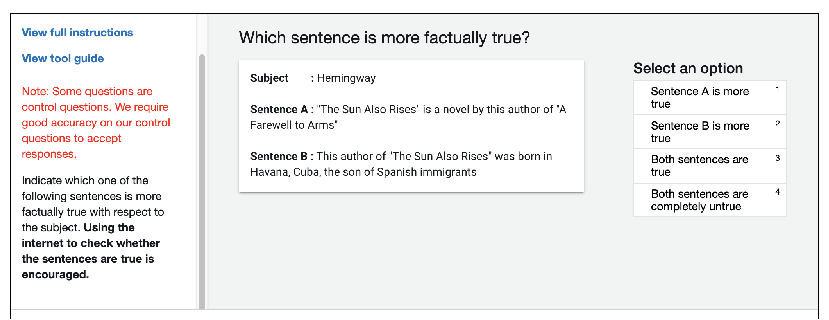
\includegraphics[width=\textwidth]{fig4_annotation.pdf}
  \caption{Giao diện chú thích cho đánh giá tính xác thực của con người. Một
  cửa sổ bật lên với hướng dẫn chi tiết và một ví dụ mẫu sẽ xuất hiện khi nhấp
  vào ``view tool guide'' (xem hướng dẫn công cụ).\\[3pt]
  {\small\textit{Ghi chú của người dịch --- nội dung giao diện:} ``Which
  sentence is more factually true?'' = \emph{Câu nào đúng sự thật hơn?}
  Chủ đề: Hemingway. Câu A: ``‘The Sun Also Rises’ là một tiểu thuyết của tác
  giả của ‘A Farewell to Arms’''. Câu B: ``Tác giả của ‘The Sun Also Rises’
  sinh ra ở Havana, Cuba, là con của những người nhập cư Tây Ban Nha''. Các lựa
  chọn: câu A đúng hơn; câu B đúng hơn; cả hai câu đều đúng; cả hai câu đều
  hoàn toàn sai. Cột trái: ``Lưu ý: Một số câu hỏi là câu hỏi kiểm soát. Chúng
  tôi yêu cầu độ chính xác tốt trên các câu hỏi kiểm soát để chấp nhận câu trả
  lời. Hãy cho biết câu nào sau đây đúng sự thật hơn đối với chủ đề. Khuyến
  khích sử dụng internet để kiểm tra xem các câu có đúng hay không.''}}
  \label{fig:annotation}
\end{figure}

Hình~\ref{fig:annotation} trình bày giao diện người dùng cho đánh giá của con
người. Để tránh mọi thiên lệch do vị trí trên màn hình, việc mô hình nào tương
ứng với câu A và câu B được chọn ngẫu nhiên cho mỗi ví dụ. Người chú thích được
khuyến khích tìm hiểu chủ đề bằng internet, và được cung cấp hướng dẫn chi tiết
cùng các ví dụ mẫu trong một thẻ hướng dẫn đầy đủ. Chúng tôi đưa vào một số câu
chuẩn (gold) để đánh giá độ chính xác của người chú thích. Hai người chú thích
đã không thực hiện tốt trên những ví dụ này và các chú thích của họ đã bị loại
khỏi kết quả.

\section{Chi tiết thiết lập huấn luyện}

Chúng tôi huấn luyện tất cả các mô hình RAG và các mô hình cơ sở BART bằng
Fairseq~\cite{b45}.\footnote{\url{https://github.com/pytorch/fairseq}} Chúng
tôi huấn luyện với số học dấu phẩy động độ chính xác hỗn hợp (mixed
precision)~\cite{b40}, phân tán quá trình huấn luyện trên 8 GPU NVIDIA V100
32GB, mặc dù việc huấn luyện và suy luận có thể chạy trên một GPU. Chúng tôi
nhận thấy việc thực hiện Tìm kiếm Tích vô hướng Cực đại với FAISS trên CPU là
đủ nhanh, vì vậy chúng tôi lưu trữ các vectơ của chỉ mục tài liệu trên CPU, đòi
hỏi khoảng ${\sim}100$ GB bộ nhớ CPU cho toàn bộ Wikipedia. Sau khi nộp bài,
chúng tôi đã chuyển mã nguồn sang HuggingFace
Transformers~\cite{b66}\footnote{\url{https://github.com/huggingface/transformers}},
đạt hiệu năng tương đương với phiên bản trước nhưng là một bản cài đặt gọn gàng
và dễ sử dụng hơn. Phiên bản này cũng được công bố mã nguồn mở. Chúng tôi cũng
nén chỉ mục tài liệu bằng các công cụ nén của FAISS, giảm yêu cầu bộ nhớ CPU
xuống 36GB. Các script để chạy thí nghiệm với RAG có thể được tìm thấy tại
\url{https://github.com/huggingface/transformers/blob/master/examples/rag/README.md}
và một bản demo tương tác của mô hình RAG có thể được tìm thấy tại
\url{https://huggingface.co/rag/}

\section{Chi tiết bổ sung về QA miền mở}
\label{app:odqa}

Đối với QA miền mở, một câu hỏi thường có nhiều chú thích câu trả lời. Các chú
thích câu trả lời này được các mô hình trích xuất khai thác trong quá trình
huấn luyện, vì thông thường tất cả các chú thích câu trả lời đều được sử dụng
để tìm các đoạn khớp trong tài liệu khi chuẩn bị dữ liệu huấn luyện. Với RAG,
chúng tôi cũng tận dụng nhiều ví dụ chú thích cho Natural Questions và
WebQuestions bằng cách huấn luyện mô hình với từng cặp $(q,a)$ riêng biệt, dẫn
đến một mức tăng nhỏ về độ chính xác. Với TriviaQA, một câu hỏi thường có nhiều
câu trả lời hợp lệ, một số trong đó không phù hợp làm mục tiêu huấn luyện,
chẳng hạn như emoji hoặc các biến thể chính tả. Với TriviaQA, chúng tôi lọc bỏ
các ứng viên câu trả lời nếu chúng không xuất hiện trong top 1000 tài liệu của
truy vấn.

\paragraph{Tiền xử lý CuratedTrec}
Các câu trả lời của CuratedTrec được cho dưới dạng biểu thức chính quy (regular
expression), điều này đã được cho là lý do khiến tập dữ liệu này không phù hợp
với các mô hình sinh câu trả lời~\cite{b20}. Để khắc phục điều này, chúng tôi
sử dụng một bước tiền xử lý, trong đó trước tiên chúng tôi truy xuất top 1000
tài liệu cho mỗi truy vấn, và sử dụng câu trả lời khớp với mẫu regex thường
xuyên nhất làm mục tiêu giám sát. Nếu không tìm thấy kết quả khớp nào, chúng
tôi dùng đến một heuristic đơn giản: sinh tất cả các hoán vị có thể có cho mỗi
regex, thay thế các ký hiệu không tất định trong cấu trúc cây lồng nhau của
regex bằng một khoảng trắng.

\paragraph{Các thiết lập đánh giá TriviaQA}
Cộng đồng QA miền mở thường sử dụng các tập dữ liệu phát triển công khai làm
tập dữ liệu kiểm thử, vì dữ liệu kiểm thử cho các tập dữ liệu QA thường bị hạn
chế và dành riêng cho mục đích đọc hiểu. Chúng tôi báo cáo kết quả sử dụng cách
chia tập dữ liệu được dùng trong DPR~\cite{b26}, nhất quán với thực hành phổ
biến trong QA miền mở. Với TriviaQA, tập dữ liệu kiểm thử này là tập TriviaQA
Web Development công khai. Roberts và cộng sự~\cite{b52} thay vào đó sử dụng
tập kiểm thử Wikipedia chính thức của TriviaQA. Févry và cộng sự~\cite{b14}
tuân theo quy ước này để so sánh với Roberts và cộng sự~\cite{b52} (xem phụ lục
của~\cite{b14}). Chúng tôi báo cáo kết quả trên cả hai tập kiểm thử để cho phép
so sánh công bằng với cả hai cách tiếp cận. Chúng tôi nhận thấy hiệu năng của
mình cao hơn nhiều khi sử dụng tập kiểm thử Wiki chính thức so với tập kiểm thử
miền mở thông thường hơn, điều mà chúng tôi cho là do các câu hỏi trong tập
kiểm thử Wiki chính thức dễ trả lời hơn từ Wikipedia.

\section{Chi tiết bổ sung về FEVER}

Với phân loại FEVER, chúng tôi làm theo cách làm từ~\cite{b32}: trước tiên sinh
lại khẳng định, sau đó phân loại dựa trên biểu diễn của trạng thái ẩn cuối
cùng, trước khi cuối cùng lấy biên trên các tài liệu để thu được xác suất của
các lớp. Tác vụ FEVER theo truyền thống có hai tác vụ con. Tác vụ thứ nhất là
phân loại khẳng định thành ``Được ủng hộ'' (Supported), ``Bị bác bỏ'' (Refuted)
hoặc ``Không đủ thông tin'' (Not Enough Info), đây là tác vụ mà chúng tôi khám
phá trong bài báo chính. Tác vụ con còn lại của FEVER liên quan đến việc trích
xuất các câu từ Wikipedia làm bằng chứng hỗ trợ cho dự đoán phân loại. Vì FEVER
sử dụng một bản kết xuất Wikipedia khác với chúng tôi, việc giải quyết trực
tiếp tác vụ này không đơn giản. Chúng tôi hy vọng sẽ giải quyết vấn đề này
trong công trình tương lai.

\section{Xác suất của tài liệu rỗng}

Chúng tôi đã thử nghiệm việc bổ sung cơ chế ``tài liệu rỗng'' (Null document)
vào RAG, tương tự như REALM~\cite{b20}, nhằm mô hình hoá các trường hợp không
thể truy xuất được thông tin hữu ích nào cho một đầu vào cho trước. Cụ thể, nếu
$k$ tài liệu được truy xuất, chúng tôi sẽ ``truy xuất'' thêm một tài liệu rỗng
và dự đoán một logit cho tài liệu rỗng này, trước khi lấy biên trên $k+1$ dự
đoán. Chúng tôi đã khám phá việc mô hình hoá logit của tài liệu rỗng bằng cách
học (i) một vectơ nhúng tài liệu cho tài liệu rỗng, (ii) một hệ số điều chỉnh
(bias) tĩnh được học, hoặc (iii) một mạng nơ-ron để dự đoán logit. Chúng tôi
không thấy các cách này cải thiện hiệu năng, vì vậy, để đơn giản, chúng tôi
lược bỏ chúng. Với Open MS-MARCO, nơi không phải lúc nào cũng truy xuất được
các tài liệu hữu ích, chúng tôi quan sát thấy mô hình học cách luôn truy xuất
một tập tài liệu cụ thể cho những câu hỏi ít có khả năng hưởng lợi từ truy
xuất, gợi ý rằng các cơ chế tài liệu rỗng có thể không cần thiết cho RAG.

\section{Tham số}

Các mô hình RAG của chúng tôi chứa các tham số có thể huấn luyện của bộ mã hoá
truy vấn và bộ mã hoá tài liệu BERT-base của DPR, mỗi bộ có 110 triệu tham số
(mặc dù chúng tôi không tự huấn luyện bộ mã hoá tài liệu), và 406 triệu tham số
có thể huấn luyện từ BART-large, 406 triệu tham số, tổng cộng là 626 triệu tham
số có thể huấn luyện. Mô hình QA miền mở ``sách đóng'' (chỉ tham số) có hiệu
năng tốt nhất là T5-11B với 11 tỷ tham số có thể huấn luyện. Mô hình T5 có số
lượng tham số gần nhất với các mô hình của chúng tôi là T5-large (770 triệu
tham số), đạt điểm 28.9 EM trên Natural Questions~\cite{b52}, thấp hơn đáng kể
so với 44.5 mà RAG-Sequence đạt được, cho thấy các mô hình lai tham số/phi tham
số cần ít tham số có thể huấn luyện hơn nhiều để đạt hiệu năng QA miền mở mạnh.
Chỉ mục bộ nhớ phi tham số không bao gồm các tham số có thể huấn luyện, nhưng
bao gồm 21 triệu vectơ 728 chiều, tương đương 15.3 tỷ giá trị. Các giá trị này
có thể dễ dàng được lưu trữ ở độ chính xác dấu phẩy động 8-bit để kiểm soát
dung lượng bộ nhớ và ổ đĩa.

\begin{table}[t]
\caption{Số lượng mẫu trong các tập dữ liệu được sử dụng. *Một tập con ẩn của
dữ liệu này được dùng để đánh giá.}
\label{tab:datasets}
\centering\small
\begin{tabular}{@{}lrrr@{}}
  \toprule
  Tác vụ & Huấn luyện & Phát triển & Kiểm thử\\
  \midrule
  Natural Questions & 79169 & 8758 & 3611\\
  TriviaQA & 78786 & 8838 & 11314\\
  WebQuestions & 3418 & 362 & 2033\\
  CuratedTrec & 635 & 134 & 635\\
  Sinh câu hỏi Jeopardy & 97392 & 13714 & 26849\\
  MS-MARCO & 153726 & 12468 & 101093*\\
  FEVER-3 lớp & 145450 & 10000 & 10000\\
  FEVER-2 lớp & 96966 & 6666 & 6666\\
  \bottomrule
\end{tabular}
\end{table}

\section{Sụp đổ truy xuất}

Trong các thí nghiệm sơ bộ, chúng tôi quan sát thấy với một số tác vụ như sinh
truyện~\cite{b11}, thành phần truy xuất sẽ ``sụp đổ'' (collapse) và học cách
truy xuất cùng những tài liệu giống nhau bất kể đầu vào là gì. Trong những
trường hợp này, một khi truy xuất đã sụp đổ, bộ sinh sẽ học cách bỏ qua các tài
liệu, và mô hình RAG sẽ hoạt động tương đương với BART. Sự sụp đổ này có thể là
do một số tác vụ có yêu cầu ít tường minh hơn về tri thức sự thật, hoặc do các
chuỗi đích dài hơn, điều có thể dẫn đến gradient ít mang thông tin hơn cho bộ
truy xuất. Perez và cộng sự~\cite{b46} cũng phát hiện các kết quả truy xuất
giả tạo (spurious) khi tối ưu hoá một thành phần truy xuất nhằm cải thiện hiệu
năng trên các tác vụ hạ nguồn.

\section{Số lượng mẫu của mỗi tập dữ liệu}

Số lượng điểm dữ liệu huấn luyện, phát triển và kiểm thử trong mỗi tập dữ liệu
của chúng tôi được trình bày trong Bảng~\ref{tab:datasets}.

% =====================================================================
%  PHẦN BỔ SUNG CỦA NGƯỜI DỊCH
% =====================================================================
\section*{Phụ lục của người dịch: Bảng đối chiếu thuật ngữ Anh -- Việt}

{\small
\begin{tabularx}{\textwidth}{@{}>{\raggedright}p{0.44\textwidth}
    >{\raggedright\arraybackslash}X@{}}
  \toprule
  Tiếng Anh & Tiếng Việt trong bản dịch\\
  \midrule
  Retrieval-Augmented Generation (RAG) & Sinh văn bản tăng cường truy xuất\\
  Knowledge-intensive tasks & Tác vụ đòi hỏi nhiều tri thức\\
  Parametric / non-parametric memory & Bộ nhớ tham số / phi tham số\\
  Pre-trained; fine-tune & Được huấn luyện trước; tinh chỉnh\\
  Retriever; generator & Bộ truy xuất; bộ sinh\\
  Query encoder; document index & Bộ mã hoá truy vấn; chỉ mục tài liệu\\
  Bi-encoder; cross-encoder & Bộ mã hoá kép; bộ mã hoá chéo\\
  Dense vector index & Chỉ mục vectơ dày đặc\\
  Maximum Inner Product Search (MIPS) & Tìm kiếm tích vô hướng cực đại\\
  Latent variable; marginalize & Biến ẩn; lấy biên\\
  Prior / posterior & Xác suất tiên nghiệm / phân phối hậu nghiệm\\
  Negative marginal log-likelihood & Log-hợp lý biên âm\\
  Beam search; greedy decoding & Tìm kiếm chùm; giải mã tham lam\\
  Thorough / Fast Decoding & Giải mã Kỹ lưỡng / Giải mã Nhanh\\
  Open-domain QA; closed-book QA & Hỏi đáp miền mở; QA sách đóng\\
  Extractive / abstractive QA & QA trích xuất / QA trừu tượng\\
  Gold passage / evidence & Đoạn văn / bằng chứng chuẩn\\
  Fact verification; claim & Kiểm chứng sự thật; khẳng định\\
  Supports / refutes / not enough info & Ủng hộ / bác bỏ / không đủ thông tin\\
  Factuality; specificity & Tính xác thực; tính cụ thể\\
  Hallucination & Ảo giác\\
  Exact Match (EM); label accuracy & Khớp chính xác; độ chính xác nhãn\\
  Ablation; frozen retriever & Thí nghiệm cắt bỏ; bộ truy xuất đóng băng\\
  Index hot-swapping & Hoán đổi nóng chỉ mục\\
  Retrieval collapse & Sụp đổ truy xuất\\
  Null document & Tài liệu rỗng\\
  Downstream task; baseline & Tác vụ hạ nguồn; mô hình cơ sở\\
  State of the art (SotA) & Tiên tiến nhất\\
  \bottomrule
\end{tabularx}
}

\end{document}
